\documentclass[spanish,a4paper,11pt]{book}
% \usepackage[spanish]{babel}
\usepackage[utf8]{inputenc}

% \usepackage{cite} % para contraer referencias

\usepackage{listings}
\usepackage{titlesec}
\usepackage{fancyhdr}
\usepackage[spanish]{babel}
\usepackage[utf8]{inputenc}

\usepackage{xcolor}
\usepackage{pdfpages}
\usepackage{url}
\usepackage{booktabs}
\usepackage[export]{adjustbox}
\usepackage{fancybox}

% \usepackage{biblatex-apa}

\usepackage[backend=biber,style=apa]{biblatex}
% \usepackage[style=numeric-comp,citestyle=apa,sorting=nyt,sortcites=true,autopunct=true,babel=hyphen,hyperref=true,abbreviate=false,backref=true,backend=biber]{biblatex}
% \usepackage{biblatex}


\usepackage[babel]{csquotes}


% \usepackage[backend=biber,style=apa]{biblatex}
\DeclareLanguageMapping{spanish-apa}
% \addbibresource{bibliography/project.bib}


% %----------------------------------------------------------------------------------------
%	BIBLIOGRAPHY AND INDEX
%----------------------------------------------------------------------------------------

% \usepackage[style=alphabetic,citestyle=numeric,sorting=nyt,sortcites=true,autopunct=true,babel=hyphen,hyperref=true,abbreviate=false,backref=true,backend=biber]{biblatex}

% \usepackage[style=numeric-comp,citestyle=ieee,sorting=nyt,sortcites=true,autopunct=true,babel=hyphen,hyperref=true,abbreviate=false,backref=true,backend=biber]{biblatex}

\addbibresource{bibliography/project.bib} % BibTeX bibliography file
\defbibheading{bibempty}{}




\usepackage{textcomp}

\usepackage{wrapfig}

\usepackage{blindtext}

\usepackage{float}

\usepackage{booktabs}

\usepackage{rotating}

\usepackage[hidelinks]{hyperref}


% Información reutilizable
\newcommand{\asunto}{Trabajo de Fin de Máster}
\newcommand{\titulo}{Autocorrección interactiva para la enseñanza y aprendizaje de la programación}
\newcommand{\tituloEng}{Interactive autocorrection for the teaching and learning of programming}
\newcommand{\master}{Máster en Profesorado de Enseñanza Secundaria Obligatoria y Bachillerato, Formación Profesional y Enseñanzas de Idiomas}
\newcommand{\autor}{Ernesto Serrano Collado}
\newcommand{\email}{info@ernesto.es}
\newcommand{\tutor}{Zoraida Callejas Carrión}
\newcommand{\escuela}{Escuela Internacional de Posgrado}
\newcommand{\universidad}{Universidad de Granada}
\newcommand{\ciudad}{Granada}
\newcommand{\vers}{Versión 0.1}
\providecommand{\keywords}{educación, enseñanza, aprendizaje, programación, integración continua, sistemas de control de versiones, software libre}

\providecommand{\keywordsen}{education, teaching, learning, programming, continuous integration, version control systems, free software}


% Información archivo
\hypersetup{
	pdfauthor = {\autor\ (\email)},
	pdftitle = {\titulo},
	pdfsubject = {\asunto},
	pdfkeywords = {\keywords},
	pdfcreator = {MacTeX con el paquete TeX Live},
	pdfproducer = {pdflatex}
}

% Estilo de cabeceras
\pagestyle{fancy}
\fancyhf{}
\fancyhead[LO]{\leftmark}
\fancyhead[RE]{\rightmark}
\fancyhead[RO,LE]{\textbf{\thepage}}
\setlength{\headheight}{1.5\headheight}

% Redefinición de comandos
\renewcommand{\lstlistingname}{Fragmento de código}
\renewcommand{\lstlistlistingname}{Índice de fragmentos de código}
\renewcommand{\chaptermark}[1]{\markboth{\textbf{#1}}{}}
\renewcommand{\sectionmark}[1]{\markright{\textbf{\thesection. #1}}}

% Definición de colores
\definecolor{gray97}{gray}{.97}
\definecolor{gray75}{gray}{.75}
\definecolor{gray45}{gray}{.45}
\definecolor{gray30}{gray}{.94}
\definecolor{lightgray}{rgb}{.9,.9,.9}
\definecolor{darkgray}{rgb}{.4,.4,.4}
\definecolor{purple}{rgb}{0.65, 0.12, 0.82}
\definecolor{background}{HTML}{EEEEEE}
\definecolor{delim}{RGB}{20,105,176}
\colorlet{punct}{red!60!black}
\colorlet{numb}{magenta!60!black}

	\definecolor{dkgreen}{rgb}{0,0.6,0}
	\definecolor{gray}{rgb}{0.5,0.5,0.5}
	\definecolor{mauve}{rgb}{0.58,0,0.82}

% Listados
\lstset{
	aboveskip=0.5cm,
	backgroundcolor=\color{gray97},
	basicstyle=\scriptsize\ttfamily,
	breaklines=true,
	%commentstyle=\color{gray45},
	frame=Ltb,
	framerule=0.5pt,
	framesep=0pt,
	framexbottommargin=3pt,
	framexleftmargin=0.1cm,
	framextopmargin=3pt,
	%keywordstyle=\bfseries,
	numberfirstline = false,
	numbers=left,
	numbersep=6pt,
	%numberstyle=\tiny,
	rulesep=.4pt,
	rulesepcolor=\color{black},
	showstringspaces = false,
	%stringstyle=\ttfamily,
	  numberstyle=\tiny\color{gray},
	  keywordstyle=\color{blue},
	  commentstyle=\color{dkgreen},
	  stringstyle=\color{mauve},
	literate={á}{{\'a}}1
	         {é}{{\'e}}1
	         {í}{{\'i}}1
	         {ó}{{\'o}}1
	         {ú}{{\'u}}1
	         {ñ}{{\~n}}1
}


% Minimizar fragmentado de listados
\lstnewenvironment{listing}[1][]
	{\lstset{#1}\pagebreak[0]}{\pagebreak[0]}

% Listado definido para JavaScript
% http://tex.stackexchange.com/questions/89574/language-option-supported-in-listings/89576#89576
\lstdefinelanguage{javascript}{
	backgroundcolor=\color{background},
	basicstyle=\footnotesize,
	breaklines=true,
	captionpos=b,
	comment=[l]{//},
	commentstyle=\color{purple}\ttfamily,
	frame=lines,
	identifierstyle=\color{black},
	keywordstyle=\color{blue}\bfseries,
	morecomment=[s]{/*}{*/},
	morestring=[b]',
	morestring=[b]",
	ndkeywordstyle=\color{darkgray}\bfseries,
	numbers=left,
	numbersep=8pt,
	numberstyle=\scriptsize,
	sensitive=false,
	showstringspaces=false,
	stepnumber=1,
	stringstyle=\color{red}\ttfamily,
	keywords={
		break,
		case,
		catch,
		catch,
		do,
		else,
		false,
		function,
		if,
		in,
		new,
		null,
		return,
		switch,
		true,
		typeof,
		var,
		while},
	ndkeywords={
		boolean,
		class,
		export,
		implements,
		import,
		this,
		throw}
}

% Listado definido para JSON
% http://tex.stackexchange.com/questions/83085/how-to-improve-listings-display-of-json-files/83100#83100
\lstdefinelanguage{json}{
	backgroundcolor=\color{background},
	basicstyle=\footnotesize,
	breaklines=true,
	captionpos=b,
	frame=lines,
	numbers=left,
	numbersep=8pt,
	numberstyle=\scriptsize,
	showstringspaces=false,
	stepnumber=1,
	literate=
		*{:}{{{\color{punct}{:}}}}{1}
		{,}{{{\color{punct}{,}}}}{1}
	    {\{}{{{\color{delim}{\{}}}}{1}
	    {\}}{{{\color{delim}{\}}}}}{1}
	    {[}{{{\color{delim}{[}}}}{1}
	    {]}{{{\color{delim}{]}}}}{1}
	    {ñ}{{\~{n}}}{1}
}

\lstdefinelanguage{yaml}{
  keywords={true,false,null,y,n},
  keywordstyle=\color{darkgray}\bfseries,
  ndkeywords={},
  ndkeywordstyle=\color{black}\bfseries,
  identifierstyle=\color{black},
  sensitive=false,
  %moredelim=[l]{}{:},
  comment=[l]{#},
  morecomment=[s]{/*}{*/},
  commentstyle=\color{purple}\ttfamily,
  stringstyle=\color{blue}\ttfamily,
  %morestring=[l]{-}{},
  morestring=[b]',
  morestring=[b]"
}

% Para que las páginas en blanco no tengan cabecera
\makeatletter
\def\clearpage{%
  \ifvmode
    \ifnum \@dbltopnum =\m@ne
      \ifdim \pagetotal <\topskip
        \hbox{}
      \fi
    \fi
  \fi
  \newpage
  \thispagestyle{empty}
  \write\m@ne{}
  \vbox{}
  \penalty -\@Mi
}
\makeatother

\begin{document}
\begin{titlepage}

\newlength{\centeroffset}
\setlength{\centeroffset}{-0.5\oddsidemargin}
\addtolength{\centeroffset}{0.5\evensidemargin}

\noindent\hspace*{\centeroffset}\begin{minipage}{\textwidth}

\centering

\includegraphics[width=0.9\textwidth]{../images/logo_ugr.png}

\textsc{\Large\asunto\\[0.8cm]}
\textsc{\master}\\[0.5cm]

{\Huge\bfseries \titulo\\}
\noindent\rule[-1ex]{\textwidth}{3pt}\\[3.5ex]
\end{minipage}

\vspace{1cm}
\noindent\hspace*{\centeroffset}\begin{minipage}{\textwidth}
\centering

\textbf{Autor}\\ {\autor}\\[2.5ex]
\textbf{Tutor}\\ {\tutor}\\[2cm]

\includegraphics[width=0.3\textwidth]{../images/logo_eip.jpg}\\[0.1cm]
\textsc{\escuela}\\
\textsc{---}\\
\ciudad, \today\\
\end{minipage}
\end{titlepage}


\frontmatter
\begin{center}
{\LARGE\bfseries\titulo}\\
\end{center}
\begin{center}
\autor\
\end{center}

\section*{Resumen}

\bigskip
\noindent{\textbf{Palabras clave}: \textit{\keywords}\\

Una de las mejores formas de aprender programación es a través de la realización de ejercicios, pero la labor de corrección de dichos ejercicios es una tarea que consume mucho tiempo. El coste de la corrección manual de ejercicios tiene una correlación directa con el número de actividades que podemos realizar con nuestros alumnos ya que a la hora de planificarlas hay que tener en cuenta el tiempo que nos va a llevar corregir dichas actividades.

\bigskip
Con herramientas y/o metodologías que nos faciliten dicha corrección podríamos proponer muchos más ejercicios e incluso generar material de extensión para alumnos con altas capacidades. Los alumnos que tengan necesidades especiales de apoyo educativo podrían hacer uso de los resultados de la corrección para entender dónde fallan. Asimismo los propios alumnos pueden ayudarse mutuamente incentivando el trabajo en equipo.

\bigskip
Vamos a proponer una metodología de trabajo que mediante el uso de sistemas de integración continua permitirá la corrección automática de ejercicios de programación reduciendo así el tiempo de corrección manual. Además los alumnos podrán ver el resultado de dicha autocorrección sirviéndoles como sistema de apoyo a su aprendizaje.

\bigskip
Para ilustrar la metodología se van a desarrollar una serie de ejercicios típicos de programación de algunos lenguajes que están incluidos en el currículo de diversas asignaturas de Educación Secundaria, Bachillerato y Formación Profesional relacionadas con la informática.


\newpage
\begin{center}
{\LARGE\bfseries\tituloEng}\\
\end{center}
\begin{center}
\autor\
\end{center}

\section*{Extended abstract}

\bigskip
\noindent{\textbf{Keywords}: \textit{\keywordsen}.\\

One of the best ways to learn computer programming is through exercises but the work of correcting such exercises is a time-consuming task. The cost of the manual correction of exercises has a direct correlation with the number of activities that we can carry out with our students, since when planning them we have to take into account the time it will take us to correct these activities.

\bigskip
With tools and/or methodologies that facilitate this correction we could propose many more exercises and even generate extension material for students with high capacities. Students with special needs for educational support could use the results of the correction to understand where they fail. Students can also help each others encouraging the work in teams.

\bigskip
We are going to propose a working methodology that through the use of continuous integration systems will allow the automatic correction of programming exercises, thus reducing manual correction time. In addition, the students will be able to see the result of this self-correction, serving them as a support system for their learning.

\bigskip
We will develop some example exercises to show how works our methodology, these exercises will be developed in the most common programming languages that are included in the curriculum of various subjects related with the computer programming.

\bigskip
There are many studies (\cite{benotti_effect_2018}) and blogs posts like \cite{noauthor_how_2019} that demostrates how  self-correction and automatic code review systems improve programming learning by allowing students to self-evaluate immediately without having to wait for the correction of the exercises. In this way the student can see the correction of the exercise when he is working on it.

\bigskip
With the classic methods of manual correction the student must wait for this correction, days or even weeks can pass until seeing where it has failed and in many cases having lost the context of what the student was trying to solve. We are going to apply some previous research and knowledge (\cite{rubio_uso_2018}) to achieve the goal of building our custom auto-correction system.


\newpage
\thispagestyle{empty}
\
\vspace{10cm}

\noindent\rule[-1ex]{\textwidth}{2pt}\\[4.5ex]

% \section*{Declaración de Originalidad del TFM}

Yo, \textbf{\autor}, alumno de la titulación \textbf{\master} de la \textbf{\escuela\ de la \universidad}, declaro que el presente Trabajo de Fin de Máster es original, no habiéndose utilizado fuentes sin ser citadas debidamente. De no cumplir con este compromiso, soy consciente de que, de acuerdo con la Normativa de Evaluación y de Calificación de los estudiantes de la Universidad de Granada de 20 de mayo de 2013, \textit{esto conllevará automáticamente la calificación numérica de cero [...] independientemente del resto de las calificaciones que el estudiante hubiera obtenido. Esta consecuencia debe entenderse sin perjuicio de las responsabilidades disciplinarias en las que pudieran incurrir los estudiantes que plagien.}

\bigskip
Asimismo, autorizo la ubicación de la siguiente copia de mi Trabajo de Fin de Máster (\textit{\titulo}) en la biblioteca del centro para que pueda ser consultada por las personas que lo deseen.

\bigskip
Además, este mismo trabajo está publicado bajo la licencia \textbf{Creative Commons Attribution-ShareAlike 4.0} \cite{CC}, dando permiso para copiarlo y redistribuirlo en cualquier medio o formato, también de adaptarlo de la forma que se quiera, pero todo esto siempre y cuando se reconozca la autoría y se distribuya con la misma licencia que el trabajo original. Todo el código fuente así como este documento en formato {\tt LaTeX} se puede encontrar en los siguientes repositorios de {\tt GitHub}: \url{https://github.com/erseco/ugr_tfm_maes} y \url{https://github.com/erseco/ugr_tfm_maes_sample_exercises}.

\bigskip
Y para que así conste firmo el presente documento.

\vspace{3cm}

\noindent Fdo: \autor

\vspace{3cm}

\begin{flushright}
\ciudad, a \today
\end{flushright}

\newpage
\thispagestyle{empty}
\
\vspace{2cm}

\noindent\rule[-1ex]{\textwidth}{2pt}\\[4.5ex]

D.ª \textbf{\tutor}, profesora del \textbf{Departamento de Lenguajes y Sistemas Informáticos} de la \textbf{\universidad}.

\vspace{0.5cm}

\vspace{0.5cm}

\textbf{Informa:}

\vspace{0.5cm}

Que el presente trabajo, titulado \textit{\textbf{\titulo}}, ha sido realizado bajo su supervisión por \textbf{\autor}, y
autoriza la defensa de dicho trabajo ante el tribunal que corresponda.

\vspace{0.5cm}

Y para que conste, expide y firma el presente informe en \ciudad\ a \today.

\vspace{1cm}

\textbf{La tutora:}

\vspace{3cm}

%\begin{figure}[H]
%\includegraphics[width=0.3\textwidth]{../../firmaZoraida}
%\end{figure}

\noindent \textbf{\tutor}

\chapter*{Agradecimientos}
\thispagestyle{empty}

\vspace{1cm}

A Georgia, que algún día será mejor ingeniera que su tío.

\bigskip
Al ZX Spectrum 128K +2A de mis hermanos, porque sin él no habría llegado hasta aquí.

\bigskip
A mi \textit{seño} Zoraida, por haber sido mi primera profesora en la carrera, por ponerme mi primera matrícula y por cerrar el círculo dirigiendo este TFM.


\begingroup
\let\cleardoublepage\clearpage
  \tableofcontents
 % \listoffigures
%  \listoftables
 % \lstlistoflistings
\endgroup

\newpage
\thispagestyle{empty}
\
\mainmatter
\chapter{Introducción}

Mi primer contacto con la informática fue a finales de los años ochenta. Un buen día mi padre apareció en casa con una caja negra y alargada que contenía un misterioso teclado que se enchufaba a la tele. En ese mismo teclado se introducía una cinta de casete como las que poníamos para escuchar música y tras esperar un rato, que ahora nos parecería una eternidad, podíamos empezar a aporrear el teclado para llevar a Phantomas (figura \ref{fig:phantomas}) de pantalla en pantalla mientras íbamos esquivando enemigos y activando las palancas que abrirían la caja fuerte de la mansión que íbamos a robar.


\begin{figure}[h!]
\centering
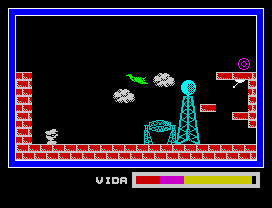
\includegraphics{../images/phantomas-sp1}
\caption{Phantomas (© 1986 Dinamic)}
\label{fig:phantomas}
\end{figure}

\bigskip
Todavía faltaba mucho tiempo para que aprendiera lo que era una interfaz (aún no había aprendido ni tan siquiera a leer) pero ya sabía interpretar algunas letras, curiosamente las que tenían pintadas las teclas OPQA\footnote{En los primeros ordenadores que aparecieron en España en la década de los 80 esta era la combinación de teclas que tenían predefinidos la mayoría de los juegos siendo OP las teclas para moverse de izquierda a derecha y QA para hacerlo de arriba a abajo.}.

\bigskip
Según fui creciendo aprendí a leer y escribir y también a reconocer unos códigos que aparecían al final de las revistas que compraba mi hermano que se llamaban POKES\footnote{Instrucción en lenguaje BASIC que graba un valor en una determinada dirección de memoria.}, estos códigos hacían que, introduciéndolos a la hora de cargar el juego, pudiera tener vidas infinitas, la habilidad de atravesar paredes o la capacidad de ser invisible a los enemigos. Estos trucos permitían a un niño torpe a los mandos, como lo era yo, el poder terminar los dificilísimos juegos de la época.

\bigskip
Pasaron algunos años y ya en el colegio muchos amigos tenían consolas de videojuegos en las que metías un cartucho e instantáneamente estabas jugando a juegos increíbles con una paleta de colores que raro era que no provocara ataques epilépticos. Mientras mis amigos solo tenían que introducir el cartucho y empezar a jugar yo tenía que esperar 5 interminables minutos mientras escuchaba sonidos estridentes y cruzar los dedos por que no apareciera el fastidioso TAPE ERROR que se podía intentar solucionar girando un tornillo llamado ``azimut'' con un destornillador que curiosamente aún poseo.

\bigskip
Y de esta manera, sin siquiera saberlo, tuve mis primeros contactos con el auto-aprendizaje, yo girando un tornillo sin saber a ciencia cierta el por qué y mis amigos el mayor problema que tenían era que a veces tenían que dar un soplido fuerte a la ranura del cartucho.

\bigskip
Mucho mas tarde entró en mi casa un flamante Pentium 166 MMX con Windows 95 OSR2 cuyo entorno tenía ventanas y era bastante intuitivo, podía escribir documentos con formato y el primo de un conocido tenía un programa te marcaba en rojo los errores ortográficos de los trabajos del colegio. De hecho ese mismo señor tenía un CD llamado Encarta donde había toda una enciclopedia metida dentro, solo tenías que escribir una palabra y al momento aparecía su definición con fotografías y todo. Ya no era necesario esperar al día siguiente para poder ojear la enciclopedia del colegio, podía obtener toda la información que necesitara mientras me quemaba las retinas con aquellos monitores de rayos de tubos catódicos.

\bigskip
Estábamos ya a mediados de 1996 y se empezaba a hablar de Internet, era como aquella Encarta pero sin CD, el futuro nuevamente había llegado y todo el dinero invertido en una grabadora de CD se iba al garete, junto con las horas mantenidas cruzando los dedos y sin tocar el ordenador para que fallara la grabación, todo estaba en Internet, y si no estaba ahí poco tardaría en estarlo.

\bigskip
Así que cogí los ahorros de mi paga semanal y me compré un módem para puerto serie de 33.000 Baudios de segunda mano. Conecté el módem metí uno de los múltiples de CDs de conexión a Internet que regalaban por aquel entonces con las revistas, le di a conectar y ahí estaban de nuevo las largas esperas escuchando ruidos estridentes igual que unos años antes.

\bigskip
A base de curiosear como buen aspirante a ingeniero vi escondido en las opciones una casilla que decía ``Silenciar altavoz'', ¿como podía ser que millones de personas estuvieran soportando esos ruidos estridente para conectarse por no saber marcar una casilla? Algo raro pasaba ya que la opción estaba ahí pero nadie la pulsaba.

\bigskip
Pasaron los años, los sistemas se fueron haciendo mas complejos y me di cuenta que según más opciones tenían los dispositivos más perezosos se volvían los usuarios. Mi vecino sin ir más lejos por no configurar su televisor tenía TVE2 en el canal 4 de su televisor ¿era yo el único que encontraba eso chirriante? Quizá no, pero como he ido descubriendo hay diferentes tipos de personas, están los que pueden pasar meses alumbrando el pasillo con el teléfono móvil y los que crean un tutorial en YouTube para enseñar a cambiar una bombilla.

\bigskip
Y ese es el deber que tenemos como futuros profesores, ser capaz de transmitir ese conocimiento e intentar que nuestros alumnos no pasen meses a oscuras, que aprendan a silenciar el volumen del altavoz del módem y en el mejor de los casos que sepamos despertar en ellos la curiosidad para que sean ellos mismos los que auto-aprendan y descubran todas esas cosas futuras que aun siendo profesores tenemos por aprender.

\section{Motivación}

Como ya sabemos Internet ha tenido un carácter académico desde prácticamente su nacimiento y por ello las mayores innovaciones y casi todo su enfoque ha salido de estos ámbitos previos a la democratización de la red y el acceso global a Internet. Es impensable concebir hoy día la enseñanza sin hacer uso de Internet y puede que en un futuro no muy lejano la totalidad de la enseñanza se imparta a través de la red.

\bigskip
La labor de un profesor no tiene un horario establecido de 8.00 a 15.00 horas, nuestra labor seguramente será 24/7 los 365 días del año y por eso tenemos que apoyarnos en herramientas que hagan nuestra vida más fácil a la vez que permiten el crecimiento exponencial de la educación.

\bigskip
Personalmente conozco profesores que han coqueteado con sistemas de mensajería instantánea (Telegram) para comunicarse con sus alumnos, dando un servicio mucho mas eficiente y rápido que las clásica tutorías.

Aplicando esa máxima de atender de una manera mas eficaz a nuestros alumnos sin que requiera una inversión adicional de nuestro tiempo...



\section{Definición del problema}


Este proyecto intentará resolver los siguientes problemas:

\begin{itemize}
  \item Evitar la tediosa tarea de la corrección de ejercicios.
  \item Motivar la enseñanza y aprendizaje de la programación a través de ejemplos.
  \item Ver cómo un sistema de control de versiones es una herramienta básica que debería enseñarse a la vez que se enseña programación.
  \item Mejorar la calidad de vida tanto de profesores como de estudiantes
\end{itemize}

\section{Estructura del proyecto}


\bigskip
Antes de pasar a detalles más técnicos, me gustaría detallar el contenido de este proyecto:

\begin{itemize}
  \item En el \textit{capítulo 1} (\textbf{Introducción}) se encuentra un texto descriptivo del proyecto, así como una breve introducción a las tecnologías que se utilizarán.\cite{QueueSystems}
  \item El \textit{capítulo 2} (\textbf{Objetivos}) detalla de forma algo más concreta los objetivos determinados que se quieren cumplir con este proyecto.
  \item En el \textit{capítulo 3} (\textbf{Metodología}) está la planificación y desarrollo de cada uno de los apartados del proyecto.
  \item En el \textit{capítulo 4} (\textbf{Resultados})se detallan todos los resultados obtenidos.
  \item En el \textit{capítulo 5} (\textbf{Conclusiones}) se pueden encontrar las conclusiones finales  así como las recomendaciones para futuros trabajos.

\end{itemize}


\bigskip
Para finalizar se incluye un anexo con el código fuente desarrollado y liberado bajo una licencia libre.


% %
% % Ejemplos de codigo LaTeX para uso futuro
% %

% \begin{figure}[h!]
% \centering
% 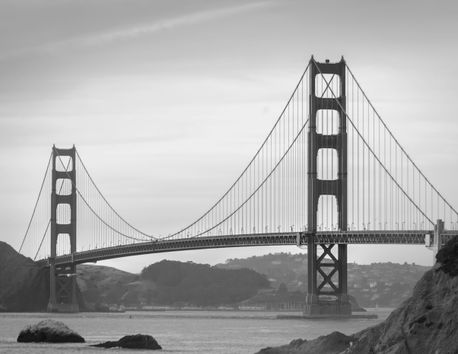
\includegraphics{../screenshots/sample1}
% \caption{Sample Image 1}
% \label{fig:sample1}
% \end{figure}

% Esto es un texto con una nota\footnote{Ejemplo de nota al pie} al pie.

% Y esto es una ``Frase de alguien''\cite{stevekrug}.

% \begin{itemize}
%   \item \textbf{1.} Texto de ejemplo
%   \item \textbf{2.} Texto de ejemplo
%   \item \textbf{3.} Texto de ejemplo
%   \item \textbf{4.} Texto de ejemplo

% \end{itemize}

% \begin{enumerate}
% 	\item Ejemplo 1.
% 	\item Ejemplo 2.
% \end{enumerate}

% \begin{lstlisting}[language=html]
% <!DOCTYPE html>
% <html lang="es-ES">
%   <head>
%     <meta charset="utf-8">
%     <title>Ejemplo de 2 párrafos</title>
%   </head>
%   <body>
%     <p>Esto es un párrafo.</p>
%     <p>Esto es otro párrafo.</p>
%   </body>
% </html>
% \end{lstlisting}

% Puedes verlo en \cite{Patricio2011}. Te recomiendo leer \cite{Patricio2011, Zacarias2009, Alfonso2010b, Alfonso2010a}.

\chapter{Objetivos}

El objetivo máximo de este proyecto es la elaboración de un sistema software que permita la autocorrección de ejercicios de programación.

\bigskip
Dicho objetivo se descompone los siguientes objetivos principales:

\begin{itemize}
  \item \textbf{OBJ-1.} Desarrollar una herramienta para la autocorrección de ejercicios de programación.
  \item \textbf{OBJ-2.} Analizar el estado del arte actual en cuanto a herramientas de autocorrección.
  \item \textbf{OBJ-3.} Analizar las posibilidades de los sistemas de autocorrección actualmente analizados.
  \item \textbf{OBJ-4.} Determinar la ventaja que nos brindan los sistemas de autocorrección para mejorar la ensañanza y aprendizaje de la programación.
\end{itemize}

Además como objetivos secundarios tendremos:

\begin{itemize}
  \item \textbf{OBJ-5.} Desarrollar una serie de ejercicios de ejemplo para comprobar el correcto funcionamiento de la herramienta.
  \item \textbf{OBJ-6.} Definir los usos posibles de la herramienta tanto para la enseñanza como para el aprendizaje de la programación.
\end{itemize}


\section{Alcance de los objetivos}
El fin inmediato de este informe es desarrollar una herramienta que permita a los profesores definir una serie de ejercicios que los propios alumnos puedan corregir de forma autonoma y automática de una forma sencilla.
Además todo el código así como la documentación resultante se liberará con una licencia libre para que cualquiera pueda hacer de la herramienta desarrollada así como de las conclusiones obtenidas.

\section{Interdependencia de los objetivos}

Todos los objetivos son interdependientes entre sí, pero el primer objetivo (\textbf{OBJ-1}) es el principal motivador de este proyecto, por lo que aún sin representar el desarrollo de ningún trabajo en concreto es el que va a escudar y avalar el desarrollo de los demás. En aspectos más relacionados con la realización del proyecto, el tercer objetivo (\textbf{OBJ-3}) es el que nos brindará el sistema sobre la que trabajar, ya que sienta la base sobre la que aplicar el cuarto objetivo (\textbf{OBJ-4}). El resto de objetivos secundarios, al no tener un carácter urgente serán resueltos en base a la disponibilidad del tiempo necesario para su realización.

\section{Conocimientos y herramientas utilizadas}

\bigskip
Destacar en los aspectos formativos previos más utilizados para el desarrollo del proyecto los conocimientos adquiridos en las asignaturas ``Cloud Computing'' para el análisis y configuración de los diferentes servicios de red así como todo lo referente a virtualización de sistemas, ``Programación Orientada a Objetos'' para el desarrollo de los ejercicios de ejemplo, ``Planificación y Gestión de. Proyectos Informáticos.'' para definir los requisitos y el planteamiento inicial del proyecto, ``Seguridad en Sistemas Operativos'' para lo referente a las buenas prácticas de programación y ``Servidores Web de Altas Prestaciones'' para la realización de pruebas desde el punto de vista de disponibilidad y carga de trabajo.

Para la realización de cada una de las partes se han usado multitud de herramientas específicas tales como pueden ser \texttt{Docker}, \texttt{Travis} \texttt{GitHub}, \texttt{LaTeX} y \texttt{git} entre otras.

\chapter{Antecedentes}

En este capítulo vamos analizar el estado de arte actual y las tecnologías candidatas a utilizarse en este proyecto en base a los objetivos que presentamos en el capítulo anterior.


\section {Procesos de verificación de código}

Existen diferentes procesos para verificar el código, los más comunes son el ``Desarrollo guiado por pruebas (TDD)'' y el ``Desarrollo guiado por comportamiento (BDD)'', ambos procedimientos tienen como finalidad verificar que el código desarrollado se adecua a los requisitos. De los dos el mas sencillo de implementar es el guiado por pruebas (\textbf{TDD}) ya que el basado en comportamiento (\textbf{BDD}) requiere de mayor capacidad de abstracción. Por ello en nuestra metodología nos basaremos en \textbf{TDD}.

\bigskip
Aun así vamos a detallar en que se basa cada uno para entender las diferencias de ambos procesos:

\subsection {Desarrollo guiado por pruebas (TDD)}

El ``desarrollo guiado por pruebas de software'' o ``Test-Driven Development (TDD)'' es una práctica de programación que consiste en dos subtareas: Primero escribir las pruebas, o \textit{Test First Development} y después refactorizar, o \textit{Refactoring}. Las pruebas son test unitarios, o \textit{unit tests}. El procedimiento es sencillo, se escribe una prueba y se verifica que fallan ya que todavía no hemos escrito el código necesario para pasar la prueba. A continuación se escribe código que hace que la prueba se ejecute sin errores y por último se refactoriza el código escrito para mejorar su desempeño y/o legibilidad.

\bigskip
El propósito del desarrollo guiado por pruebas es lograr que nuestro código funcione y a la vez sea sencillo y legible. La idea es que los requisitos sean traducidos a pruebas, de este modo, cuando las pruebas pasen se garantizará que el software cumple con los requisitos que se han establecido. Como se indica en Clean Code: `Writing clean code is what you must do in order to call yourself a profesional. There is no reasonable excuse for doing anything less than your best'' (\cite{martin_clean_2009}).

\subsection {Desarrollo guiado por comportamiento (BDD)}

El ``desarrollo guiado por comportamiento'', o ``Behavior-Driven Development (BDD)'' es una práctica de programación que surgió a partir del \textfb{TDD}. Combina las técnicas generales y los principios del TDD junto con prácticas de análisis y diseño orientado a objetos para establecer herramientas que en teoría puedan utilizarse por equipos externos al de desarrollo para definir los test, sin implicar que ese equipo externo tenga conocimientos de programación. E e y un proceso compartido de colaboración en el desarrollo de software.

\bigskip
A pesar de su definición teórica, la capacidad de abstracción necesaria para escribir buenos test basados en el comportamiento hace que en la mayoría de casos se necesite de conocimientos avanzados de programación.


\section {Herramientas de verificación de código}

Las herramientas de verificación de código se utilizan para realizar los procesos anteriormente descritos, pasamos a enumerar las más comunes:

\subsection {Pytest}

Pytest es un framework de test unitarios para el lenguaje de programación Python que facilita la creación de pruebas sencillas y escalables. Las pruebas son expresivas y legibles y no se requieren código adicional.

\subsection {PEP8}

PEP8 es una guía de estilo de codificación para Python definida por sus creadores y que está definida como el estilo estándar del lenguaje.

\subsection {RSpec}

RSpec es una herramienta para realizar test BDD que sirve para probar código escrito en el lenguaje de programación Ruby. Se utiliza ampliamente en aplicaciones de producción.

\subsection {Tidy}

HTML Tidy es una aplicación de consola que sirve para corregir código HTML no válido, detectar posibles errores de accesibilidad web y mejorar el diseño y el estilo de sangría del marcado resultante. Fue desarrollado en 2002 por Dave Raggett, miembro del World Wide Web Consortium (W3C).

\section {Herramientas interactivas de corrección}

Existen diversas herramientas de corrección de código que funcionan de forma interactiva, vamos a enumerar las principales:

\subsection {Coderunner}

CodeRunner es un plugin gratuito de código abierto para Moodle que permite ejecutar el código fuente escrito por los estudiantes en respuesta preguntas de programación en muchos lenguajes diferentes. Está pensado principalmente para su uso en cursos de programación informática aunque puede utilizarse para calificar cualquier pregunta cuya respuesta sea texto. Su funcionamiento es tal que a una pregunta concreta sobre programación el estudiante deben escribir el código fuente en respuesta. Tras ello el código pasa a ejecutarse y pueden ver los resultados inmediatamente. Los estudiantes pueden corregir su código y volver a enviarlo, normalmente a cambio de una pequeña penalización. Coderunner se puede obtener desde el sitio \url{https://coderunner.org.nz}

\subsection {Python Tutor}

Python Tutor es una herramienta de visualización de programas basada en web para Python, ya que dicho lenguaje se está convirtiendo en un lenguaje popular para la enseñanza de cursos introductorios de programación. Con esta herramienta, los profesores y los alumnos pueden escribir programas de Python directamente en el navegador web (sin instalar ningún complemento), avanzar y retroceder a través de la ejecución para ver el estado de las estructuras de datos en tiempo de ejecución y compartir sus visualizaciones de programas en la web.

En los últimos tres años, más de 200,000 personas han usado Python Tutor para visualizar sus programas \cite{GuoSIGCSE2013}. Además, los instructores de más de una docena de universidades como UC Berkeley, MIT, la Universidad de Washington y la Universidad de Waterloo lo han utilizado en sus cursos de ciencias de la computación. Python Tutor es un software gratuito y de código abierto, se puede obtener desde \url{http://pythontutor.com}.


\subsection {Jupyter Notebooks}

Jupyter Notebook (anteriormente IPython Notebooks) es un entorno basado en la web para la creación de documentos interactivos. El término ``cuaderno'' puede hacer referencia coloquialmente a muchas entidades diferentes, principalmente la aplicación web Jupyter, el servidor web Jupyter o el formato de documento Jupyter dependiendo del contexto. Un documento Jupyter Notebook es un documento JSON, siguiendo un esquema versionado, y conteniendo una lista ordenada de celdas de entrada/salida que pueden contener código, texto (usando Markdown), matemáticas, gráficos y medios enriquecidos, normalmente terminando con la extensión ``.ipynb''. El proyecto Jupyter está licenciado bajo la BSD por lo que uso y distribución es gratuito, se puede obtener desde \url{https://jupyter.org}

\subsection {Turingscraft's CodeLab}

Esta herramienta comercial es la única de la lista que no tiene una licencia libre, está desarrollada por la empresa Neoyorquina Turingcrafts y desde 2002 ha sido utilizada por más de trescientos mil estudiantes de 20 países distintos \cite{barr_using_2016}. Se puede obtener más información desde su web \url{http://www.turingscraft.com/}



\chapter{Propuesta Pedagógica}

En este capítulo pasamos a detallar la ventaja pedagógica que se pretende obtener en en base a los objetivos que presentamos en el segundo capítulo y a los antecedentes vistos en el tercero.



\section{Análisis de las soluciones}

% Primero tendrías que decir que la solución a todos los males comentados es tener una forma de integración continua y por qué, después decir qué alternativas hay

Nos gustaría proponer una metodología donde los alumnos usen herramientas que van a tener que usar en futuro profesional (o académico) como pueden ser los sistemas de control de versiones y los sistemas de integración continua, o \textit{continuous integration (CI)}, hay que tener en cuenta que esta metodología está enfocada mayoritariamente a la Formación Profesional porque es la que más asignaturas relacionadas con la programación, como veremos más adelante. Como la finalidad Formación Profesional es enseñar una profesión enseñarles a nuestros alumnos a usar estos sistemas les va a ser de gran ayuda a la hora de conseguir empleo.

\bigskip
Las tres soluciones libres descritas en los antecedentes (Coderunner, Python Tutor y Jupyter Notebooks) obligan a nuestros alumnos a aprender a usar una herramienta concreta que posiblemente no vayan a volver a utilizar jamás. Esto sería comparable a lo que didácticamente decimos de que el alumno ``aprende a aprobar exámenes'' mas que aprender los contenidos de la asignatura.

\bigskip
Por eso hemos optado por utilizar dos de las tecnologías más utilizadas para gestión de código fuente e integración continua como pueden ser GitHub y Travis CI. Además, ambas son de uso gratuito para proyectos de software libre, fomentando así su uso como se indica en la Orden de 21 de febrero de 2005, sobre disponibilidad pública de los programas informáticos de la Administración de la Junta de Andalucía y de sus Organismos Autónomos.

\section {Temario relacionado con la programación informática}

Tal y como indica el Decreto 110/2016  de 14 de junio, por el que se establece la ordenación y el currículo del Bachillerato en la Comunidad Autónoma de Andalucía las tecnologías de la información y de la comunicación para el aprendizaje y el conocimiento se utilizarán de manera habitual como herramientas integradas para el desarrollo del currículo. Asimismo en los currículos de las distintas ramas educativos donde podemos ejercer como profesores incluyen asignaturas relacionadas con la informática y de forma más específica con la programación informática.


\bigskip
\textit{``Tecnologías de la Información y Comunicación es un término amplio que enfatiza la integración de la informática y las telecomunicaciones, y de sus componentes hardware y software, con el objetivo de garantizar a los usuarios el acceso, almacenamiento, transmisión y manipulación de información. Su adopción y generalización han provocado profundos cambios en todos los ámbitos de nuestra vida, incluyendo la educación, la sanidad, la democracia, la cultura y la economía, posibilitando la transformación de la Sociedad Industrial en la Sociedad del Conocimiento.''} \cite{junta_de_andalucia_decreto_2016}

\bigskip
La oferta de asignaturas de informática es variopinta, pues en la Educación Secundaria y Bachillerato es muy básica pero muy específica en la Formación Profesional, por lo que es complejo tener una metodología que se adapte a todos los niveles. Asimismo, los temarios suelen ser bastante extensos incluyendo tanto contenido que es muy difícil abordar cada tema en profundidad. Aquí podemos ver una de las ventajas de nuestra propuesta ya que por un lado, el tiempo que ahorramos lo podemos invertir en impartir más contenidos y que podemos centrarnos en las partes donde fallan los alumnos al ver el histórico de sus errores.

\bigskip
A continuación vamos a enumerar las distintas asignaturas relacionadas con la informática que se pueden encontrar en los currículos de Educación Secundaria, Bachillerato y Formación Profesional, además indicaremos cuales son candidatos a utilizar nuestra metodología en base a sus contenidos.

\subsection {Educación Secundaria Obligatoria (ESO)}

En la Orden de 14 de julio de 2016 se especifica el currículo de la materia de ``Tecnologías de la Información y Comunicación'' que es una materia de opción del bloque de asignaturas específicas para el alumnado de cuarto curso de la Educación Secundaria Obligatoria. Es una asignatura de carácter optativo que intenta dar una visión global de la informática, con lo que su temario intenta abarcar desde historia de la informática hasta la seguridad o la programación web pasando por la ofimática y estudio de los elementos de hardware, nuestra metodología propuesta podría servir de ayuda para la enseñanza de programación de páginas web con HTML que es uno de los contenidos que se dan en dicha asignatura.

\subsection {Bachillerato}

En la Orden de 14 de julio de 2016, por la que se desarrolla el currículo correspondiente al Bachillerato en la Comunidad Autónoma de Andalucía indica las diferentes modalidades de bachillerato, incluyendo las modalidades de Ciencias y la de Humanidades y Ciencias Sociales las asignaturas de carácter obligatorio ``Tecnologías de la Información y de la Comunicación I'' y ``Tecnologías de la Información y de la Comunicación II'' y habiendo también una asignatura de libre configuración autonómica llamada ``Programación y Computación''. Estas asignaturas contienen contenidos de programación informática y de programación de páginas web por lo tanto son susceptibles de utilizar nuestra metodología de realización de ejercicios.

\subsection {Ciclo Formativo Grado Medio (CFGM)}

La Orden EDU/2187/2009, de. 3 de Julio establece el currículo del ciclo formativo de Grado Medio correspondiente al título de ``Técnico en Sistemas Microinformáticos y Redes (SMR)'' que es el único ciclo de grado medio relacionado con la informática donde la única asignatura ligeramente relacionada con la programación es ``Aplicaciones web'', pero dicha asignatura se centra más en el despliegue de aplicaciones que en la programación en sí, por lo que aunque nuestra metodología se podría adaptar para enseñar a configurar como desplegar aplicaciones web no entra dentro del alcance de este trabajo por lo que se deja como posible trabajo futuro.

\subsection {Ciclo Formativo Grado Superior (CFGS)}

Existen tres ciclos formativos de grado superior del plan LOE relacionados con la informática, la Orden EDU/392/2010, de 20 de enero, por la que se establece el currículo del ciclo formativo de Grado Superior correspondiente al título de ``Técnico Superior en Administración de Sistemas Informáticos en Red'' describe las asignaturas ``Lenguajes de Marca y Sistemas de Gestión de Información'' y ``Gestión de Bases de Datos'' en las que nuestra metodología se puede aplicar para corregir los ejercicios ya que se enseñan los lenguajes HTML, SQL, Javascript, XML así como algunos subconjuntos de XML como son DTD y XSD. Los currículos del título de ``Técnico Superior en Desarrollo de Aplicaciones Web'' definido en la Orden EDU/2887/2010, de 2 de noviembre y el de ``Técnico Superior en Desarrollo de Aplicaciones Multiplataforma'' definido en la Orden EDU/2000/2010, de 13 de julio definen varias asignaturas, algunas comunes, como pueden ser ``Programación'', ``Bases de Datos'' y ``Lenguajes de marcas y sistemas de gestión de información'' y otras específicas de cada título como pueden ser ``Programación multimedia y dispositivos móviles'' o ``Desarrollo web en entorno cliente'' que están centradas en el aprendizaje de la programación informática y en los que si encajaría nuestra metodología.

\subsection {Formación Profesional Básica (FPB)}

La Orden ECD/1030/2014, de 11 de junio define el ``Título Profesional Básico en Informática y Comunicaciones'' y la Orden ECD/1633/2014, de 11 de septiembre define el  ``Título Profesional Básico en Informática de Oficina'', siendo ambas titulaciones las únicas relacionadas con la informática de todas las que componen la formación profesional básica, pero al igual que con el ciclo formativo de Grado Medio ambos currículos carecen de temario específico de programación por lo que queda fuera del ámbito de este proyecto.


% Sería interesante que después de esto destacases la complejidad de tener una metodología de trabajo que permita cubrir los diferentes niveles de complejidad y conceptos que los estudiantes deben aprender, y cómo afrontas ese reto. También puedes decir que la mayoría de temarios (especialmente el de bachillerato) están muy sobrecargados de contenidos lo que resta tiempo para hacer mucha variedad de ejercicios en clase, lo que apoya tu propuesta... En definitiva, que saques de toda esta descripción cosas en claro que apoyen tu visión


\section{Encuesta de percepción}

Se realizó una breve encuesta y se difundió entre algunos profesores de diferentes ámbitos con el fin de ver si nuestra hipótesis de que la corrección de ejercicios era la tarea más tediosa que realizaban como docentes.

\bigskip
Aprovechamos la encuesta para obtener también algunos datos interesantes sobre la forma de trabajar de los docentes, de cara a trabajos futuros. La encuesta se podía consultar en la siguiente dirección web: \url{https://forms.gle/xxSz6mQDjswo5B137}.

\bigskip
La encuesta estuvo activa desde el 19 hasta el 25 de Mayo de 2019 y se recopilaron un total de 47 respuestas. Es una población pequeña pero aun así es interesante por las características de la misma ya que la encuesta se compartió ``de boca a oreja'' indicando que sólo lo compartieran con otros profesores a ser posible relacionados con la informática para no desvirtuar las respuestas.


\begin{enumerate}

\item \textbf{¿Dónde sueles impartir tus clases?}

Con esta pregunta queríamos tener una visión de la población encuestada, ya que al difundirla entre profesores y animarles a compartirla entre sus compañeros profesores era muy posible que sus red de contactos no se limitara a profesores de Educación Secundaria, así que dejamos elegir entre las siguientes opciones:

\begin{itemize}
    \item Educación Primaria
    \item Educación Secundaria
    \item Universidad (Grado/Máster)
    \item Practicas MAES
\end{itemize}

\bigskip
La gran mayoría de los encuestados han resultado ser profesores de Educación Secundaria, por lo que los resultados han sido satisfactorios, los siguientes han sido estudiantes en prácticas en el \master los cuales podríamos englobar dentro del conjunto de los de Secundaria, llegando así casi al 90\% de la población encuestada. Le siguen la respuestas de algunos profesores de Universidad y por último algunos maestros de Educación Primaria.

\begin{figure}[H]
\centering
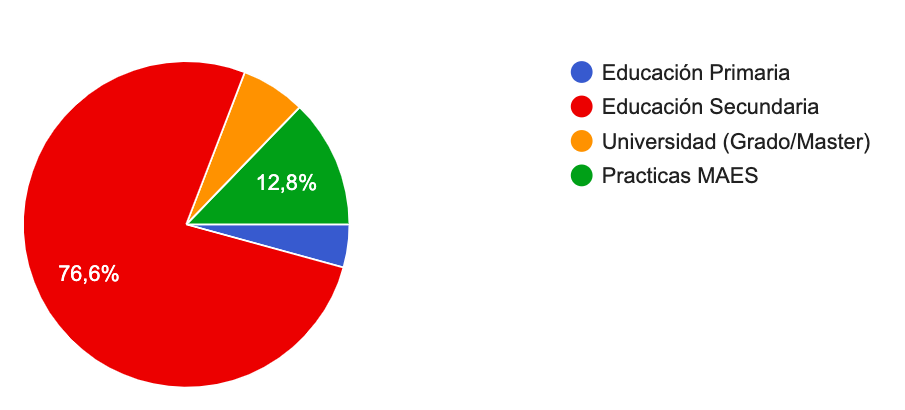
\includegraphics[width=1.0\textwidth]{../images/quiz_1}
\caption{¿Dónde sueles impartir tus clases?}
\label{fig:quiz_1}
\end{figure}


\item \textbf{Valora las siguientes tareas que sueles realizar}

Esta es quizá la pregunta más importante de toda la encuesta, porque queríamos saber la opinión de diversos profesores sobre las tareas de corrección de ejercicios y/o exámenes. Además nos ha servido para hacernos una idea de lo que opinan de las tareas más comunes de un profesor, había que valorarlas según se consideraban ``divertidas'', ``normales'' o ``tediosas'' entendiéndose tediosas como aburridas. Las opciones eran las siguientes:

\begin{itemize}
    \item Preparación de material
    \item Preparación de clases
    \item Impartir clases
    \item Corrección de ejercicios
    \item Evaluación final
    \item Tutorías
\end{itemize}

Como podemos ver, la hipótesis de que corregir ejercicios resulta tedioso ha sido validada. De hecho ha sido la única de las opciones que no ha recibido ningún voto como actividad ``divertida''. Del resto de preguntas podemos deducir que a la mayoría de profesores les divierte impartir clases, esto es algo normal. No tendría sentido una respuesta diferente dado el carácter vocacional de la profesión, y si nos centráramos en los aspectos económicos es más flagrante en el mundo de la informática porque los sueldos de la empresas privadas están muy por encima de lo que se puede llegar a cobrar como docente. El resto de preguntas se han considerado normales, habiendo opiniones en las tres vertientes. Quizá remarcar que la evaluación es la que menos votos de tarea ``divertida'' han recibido. Aunque esto puede variar mucho de un centro a otro.

\begin{figure}[H]
\centering
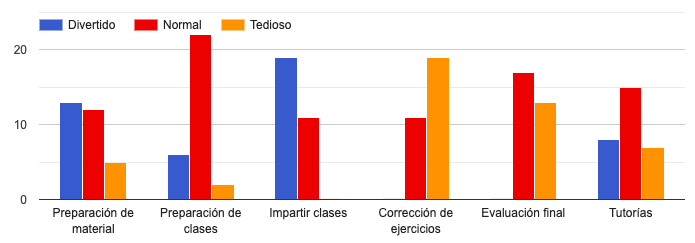
\includegraphics[width=1.0\textwidth]{../images/quiz_2}
\caption{Valora las siguientes tareas que sueles realizar}
\label{fig:quiz_2}
\end{figure}

\item \textbf{¿Elaboras tus propios ejercicios?}

En esta pregunta queríamos saber si los profesores elaboran sus propios ejercicios. En mi experiencia como alumno así como en mi experiencia como docente en prácticas he visto exactamente lo que se ve reflejado en la encuesta, hay profesores que elaboran todo su material, los hay que lo hacen de forma regular pero no siempre, también los hay que los realizan de forma ocasional. Aquí me gustaría remarcar que la opción ``Nunca'' ha recibido muy pocos votos cuando en mi experiencia también hay docentes que utilizan el material de otros profesores en lugar del suyo propio.

\begin{figure}[H]
\centering
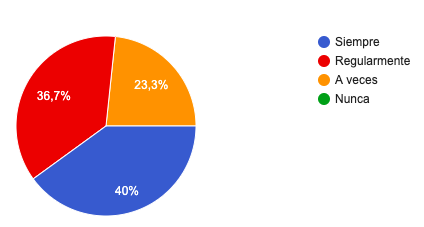
\includegraphics[width=1.0\textwidth]{../images/quiz_3}
\caption{¿Elaboras tus propios ejercicios?}
\label{fig:quiz_3}
\end{figure}

\item \textbf{¿Crees que hay que compartir los ejercicios con el resto de la comunidad?}

Esta pregunta era para ver la repercusión que tiene a nivel docente los conceptos del software libre y las licencias abiertas como la GPL y la ``Creative Commons'' \cite{comons_creative_2013} así como la WikiPedia y otros proyectos que abogan por la difusión libre y gratuita tanto de software como de todo tipo de contenidos culturales.

\bigskip
Por nuestra experiencia pensábamos que no iba a haber tan buena acogida del ``Sí'' como ha habido, pero nos ha sorprendido gratamente que la gran mayoría de los profesores encuestados apoyen el compartir el material. También es algo que se puede considerar normal ya que hoy en día es difícil hacer uso de recursos de terceros encontrados online para apoyar nuestras clases. De hecho en mi periodo como docente en prácticas me sirvió para ver que al contrario que en mi época de estudiante, donde usábamos el libro de texto, los docentes usan recursos como Kahoot!\footnote{Plataforma gratuita que permite la creación de cuestionarios de evaluación en forma de concurso.} o YouTube para hacer las clases mucho más dinámicas.

\begin{figure}[H]
\centering
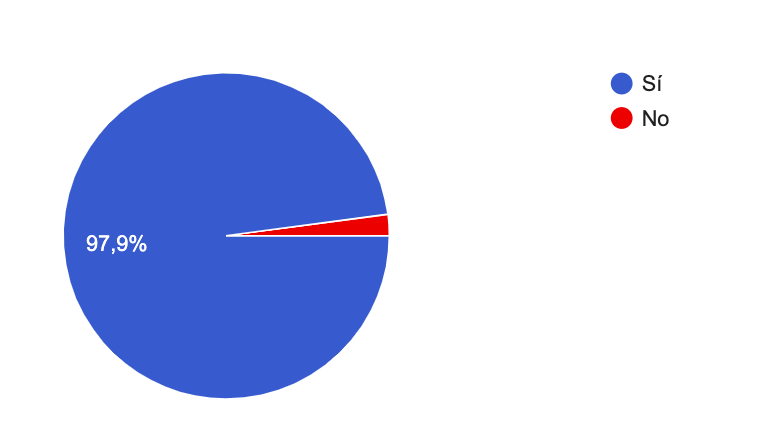
\includegraphics[width=1.0\textwidth]{../images/quiz_4}
\caption{¿Crees que hay que compartir los ejercicios con el resto de la comunidad?}
\label{fig:quiz_4}
\end{figure}

\item \textbf{¿Sueles entregar correcciones de los ejercicios?}

Esta pregunta está íntimamente relacionada con el propósito de este trabajo, queríamos saber si los profesores solían entregar los ejercicios corregidos, hay que tener en cuenta que para que dicha corrección tenga utilidad las correcciones se han de entregar de forma temprana, ya que es cuando el alumno aun está adquiriendo los conocimientos, de dieron las opciones ``Sí'', ``No'' y ``Otra'', siendo esta última opción para que los profesores indicaran alguna opción distinta, a continuación se pega en bruto dichas opciones alternativas:

\begin{itemize}
    \item Algunas veces
    \item A veces y otras se corrigen en clase.
    \item Sí o se corrigen en clase.
\end{itemize}

Nos pareció interesante la opción de la corrección en clase, pues no la habíamos tenido en cuenta, pensamos que es una forma muy didáctica de que el alumno vea dónde ha fallado y hacer una corrección temprana, pero teniendo en cuenta que por norma general siempre hay una sensación de falta de tiempo para impartir el temario, así que quizá invertir tiempo en esta corrección puede hacer que lo perdamos para impartir nuevos contenidos.

\begin{figure}[H]
\centering
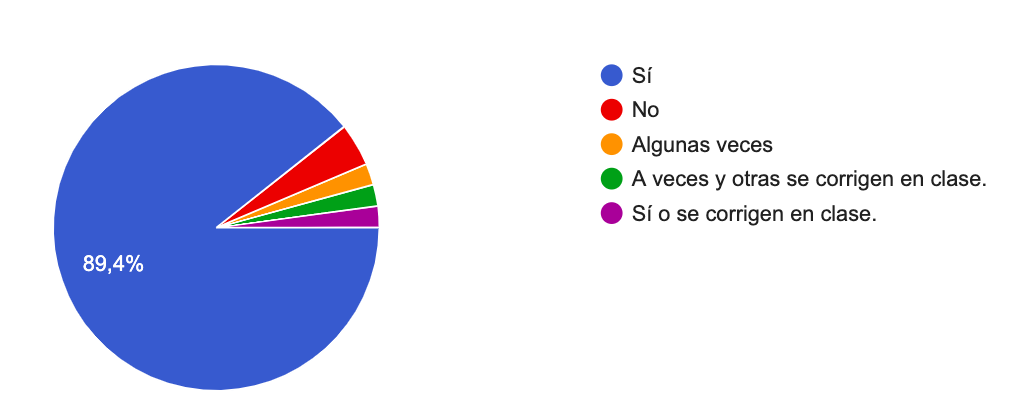
\includegraphics[width=1.0\textwidth]{../images/quiz_5}
\caption{¿Sueles entregar correcciones de los ejercicios?}
\label{fig:quiz_5}
\end{figure}

\item \textbf{¿Qué opinas de los sistemas de corrección automática?}

Aquí preguntamos de forma directa sobre los sistemas de corrección automática de forma genérica, sin especificar ninguno, ya que como hemos visto en los antecedentes existen diversos métodos, aquí les dimos a elegir entre estas opciones:

\begin{itemize}
    \item Ahorran tiempo a alumnos y profesores
    \item Mejoran la enseñanza al poder ver de manera más inmediata los resultados
    \item Desvirtúan la finalidad de los ejercicios propuestos
    \item Deshumaniza la relación profesor-alumno
    \item Otra (especificar)
\end{itemize}

La opción ``Mejoran la enseñanza al poder ver de manera más inmediata los resultados'' fue marcada por casi el 50\% de los encuestados, seguida por la de ``Ahorran tiempo a alumnos y profesores'' que consiguió algo más del 20\%, ambas en conjunto eran las opciones que eran más acordes al desarrollo de nuestra metodología por lo que podemos ver que hay un claro interés en estos sistemas, además pusimos la opción ``Otra'' donde los profesores indicaron opiniones adicionales que pasamos a enumerar:

\begin{itemize}
    \item Ahorran tiempo a todos y mejoran la enseñanza. Se pueden hacer más ejercicios y practicar mucho es esencial en enseñanzas técnicas.
    \item Sirven para ver si los alumnos han adquirido los conocimientos.
    \item Es otro tipo de herramienta de evaluación.
    \item No lo he probado.
    \item Son útiles en su justa medida.
\end{itemize}

En estas respuestas vemos que en su mayoría también coinciden que los sistemas de corrección automática son muy útiles para mejorar la enseñanza, así que creemos que esta propuesta metodológica puede ser de gran ayuda a profesores.

\begin{figure}[H]
\centering
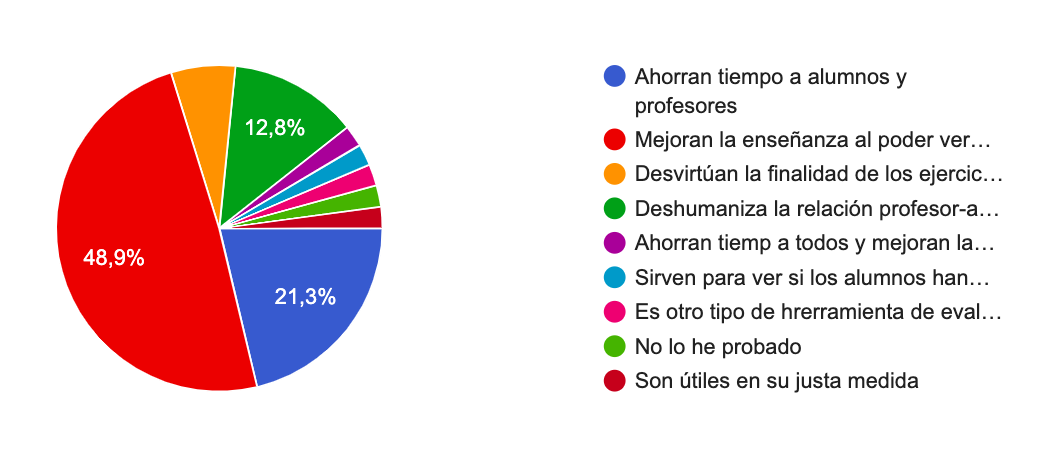
\includegraphics[width=1.0\textwidth]{../images/quiz_6}
\caption{¿Qué opinas de los sistemas de corrección automática?}
\label{fig:quiz_6}
\end{figure}

\item \textbf{Sugerencias para mejorar las clases}

Incorporamos a la encuesta un apartado para que los profesores aportaran sus sugerencias para mejorar las clases, a continuación vamos a poner los datos recopilados en bruto en dicho apartado:

\begin{itemize}
    \item Hacerlas dinámicas y participativas, huir de la explicación meramente.
    \item Lo más eficiente para el aprendizaje del alumnado es que ellos mismos corrijan, así si se les indican los errores suelen verlos y evitarlos después.
    \item Que parte de la evaluación la hagan los propios alumnos (son más conscientes de los errores cometidos).
    \item Fomentar el trabajo basado en proyectos colaborativos.
    \item Correcciones en clase de la totalidad de los ejercicios, haciendo partícipes a los alumnos.
    \item Coevaluación, aula invertida. Cooperativo.
    \item Participación continuada de alumno.
    \item La tipología de ejercicio más eficiente a la hora de su corrección es el tipo test. Existe una optimización de tiempo de corrección bastante notable en comparación con ejercicios con preguntas de desarrollo, donde se tarda más por no tener tan automatizada la respuesta correcta (hay que leer la respuesta), la puntuación se somete a matices por estar incompleta, en ocasiones es difícil comprender la letra del alumno, etc.
\end{itemize}


\end{enumerate}

\section{Definición de la metodología}

% ok con que contrastas con el test, pero me falta lo que te comentaba antes que metieses en otras secciones: una discusión acerca de la naturaleza de los ejercicios, por qué es útil emplear una solución como la tuya, etc.

Tras validar que nuestra propuesta efectivamente tiene un alto valor pedagógico y que encaja dentro de los contenidos de varias asignaturas de los currículos de educación secundaria pasamos a definir los objetivos, contenidos y competencias de nuestra metodología.

\bigskip
El objetivo de nuestra metodología es enseñar programación de una forma diferente, con ejercicios, autocorrección y con tecnologías que se usan en el día a día de cualquier informático que se dedique profesionalmente a ello. La misma nos brinda muchas ventajas como puede ser ver un histórico de los envíos de un alumno, para saber donde falla o el tiempo que le ha dedicado a un ejercicio concreto, un simple vistazo al ``Travis CI'' de cada alumno nos da mucha información, y el poder seguir la traza es muy útil, también podemos ver el historial de \textit{commits} de \textit{Git} de forma rápida para ver la evolución del alumno. El código de colores de \textit{Travis CI} también hace que corregir sea intuitivo, verde para correcto y rojo para incorrecto. En un momento dado podríamos detectar un posible plagio entre alumnos de forma rápida usando el mencionado historial.

\bigskip
Como indica el Decreto 110/2016  de 14 de junio el alumno debe \textit{``conocer el funcionamiento de las nuevas tecnologías de la información y la comunicación, comprendiendo sus fundamentos y utilizándolas para el tratamiento de la información (buscar, almacenar, organizar, manipular, recuperar, presentar, publicar y compartir), así como para la elaboración de programas que resuelvan problemas tecnológicos''} (\cite{junta_de_andalucia_decreto_2016}), así que además de todo lo indicado anteriormente estamos ajustándonos a la normativa.

\bigskip
El decreto anteriormente citado dice que ``la oferta curricular diseñada en este Decreto potencia el desarrollo de las tecnologías de la información y la comunicación, así como la enseñanza de las lenguas extranjeras, teniendo en cuenta los objetivos emanados de la Unión Europea en esta materia y los planes estratégicos de la Comunidad Autónoma de Andalucía para el desarrollo de las lenguas'' por lo que todos los ejercicios propuestos han sido realizados en inglés ya que es el idioma predominante en la informática y nuestros alumnos deberán adquirir competencias de lectura y comprensión en lengua inglesa para poder aprender por si mismos, de hecho el comando \textit{Git} y las páginas \textit{GitHub}, \textit{Travis CI} están completamente en inglés así como la mayor parte de la documentación de lenguajes de programación. Sin ir más lejos la propia programación informática define sus directivas en inglés, con palabras como ``function'', ``class'' ``for'', ``if'', ``then'' o ``while''.

\subsection{Contenidos}

Los contenidos de nuestra metodología comprenderán dos partes. Una parte común a todas las asignaturas donde se enseñará a usar Git y algunos conceptos básicos de programación y otra específica donde haciendo uso de lo aprendido en la parte común se seguirá el temario de la asignatura en cuestión.

% Eso de que la introducción a la programación se pueda poner o quitar es muy relativo, explícalo mejor

\bigskip
La parte común comprenderá los siguientes dos apartados que se definirán de modo más extenso en la propuesta metodológica:

\begin{itemize}
    \item Aprendiendo a usar Git: Comandos básicos, creación de una cuenta en GitHub, integración continua, realizar un \textit{fork} del repositorio de ejercicios ...
    \item Introducción a la programación: Conceptos comunes a todos los lenguajes como ``variable'' y ``constante'', condicionales y bucles,...
\end{itemize}

Esta parte común podrá resumirse o incluso obviarse si los alumnos ya conocen alguno de los dos conceptos básicos por haberlos aprendido en otra asignatura.

\bigskip
La parte específica se desarrollará en base a los contenidos de la asignatura a impartir, pero en la propuesta metodológica se definirán algunos ejercicios de ejemplo de diferentes asignaturas como pueden ser ``Lenguajes de marcas y sistemas de gestión de información'', ``Programación'' o ``Bases de Datos''.

\bigskip
Los ejercicios de la parte específica estarán siempre disponibles en su totalidad para que los alumnos puedan ir avanzando al ritmo que deseen. Cada ejercicio tendrá una breve explicación de lo que se requiere y una serie de test TDD que deberán pasar. El profesor también podrá poner ejercicios resueltos pero con algunos errores para que los alumnos los corrijan.

\subsection{Competencias}

La programación informática, y por extensión nuestra metodología, permite adquirir las siguientes 5 del total de 7 competencias clave de la LOMCE descritas en la Orden ECD/65/2015, de 21 de enero:

\begin{itemize}
    \item \textbf{CCL}: Competencia en comunicación lingüística
    \item \textbf{CMCT}: Competencia matemática y competencias básicas en ciencia y tecnología
    \item \textbf{CD}: Competencia Digital
    \item \textbf{CPAA}: Competencia de aprender a aprender
    \item \textbf{SIE}: Sentido de la iniciativa y espíritu emprendedor
\end{itemize}

Entrando en detalle, de nuestra metodología, podemos destacar y definir las siguientes tres:

\begin{itemize}

    \item Utilizar las tecnologías de la información y la comunicación de modo habitual en el proceso de aprendizaje, buscando, analizando y seleccionando información relevante en Internet o en otras fuentes,  elaborando documentos propios, haciendo exposiciones y argumentaciones de los mismos y compartiendo éstos en entornos apropiados para facilitar la interacción.

    \item Conocer el funcionamiento de las nuevas tecnologías de la información y la comunicación, comprendiendo sus fundamentos y utilizándolas para el tratamiento de la información (buscar, almacenar, organizar, manipular, recuperar, presentar, publicar y compartir), así como para la elaboración de programas que resuelvan problemas tecnológicos.

    \item Asumir de forma crítica y activa el avance y la aparición de nuevas tecnologías, incorporándolas al quehacer cotidiano.

\end{itemize}

\subsection{Proceso de entrega}
Para la entrega de ejercicios el alumno deberá realizar un ``Pull request'' contra el repositorio del profesor lo cual dará el ejercicio por entregado. El repositorio tiene una plantilla para la creación de dichos \textit{pull requests} en la que al alumno comprobará un checklist indicando que ha leído el guión de la práctica, cumple los posible pre-requisitos (por ejemplo haber terminado un ejercicio previo) así como indicar que el código entregado es original y no ha tratado de hacer modificaciones en el TDD ni en el \textit{pipeline} (figura \ref{fig:github_pr_create}).

\begin{figure}[h!]
\centering
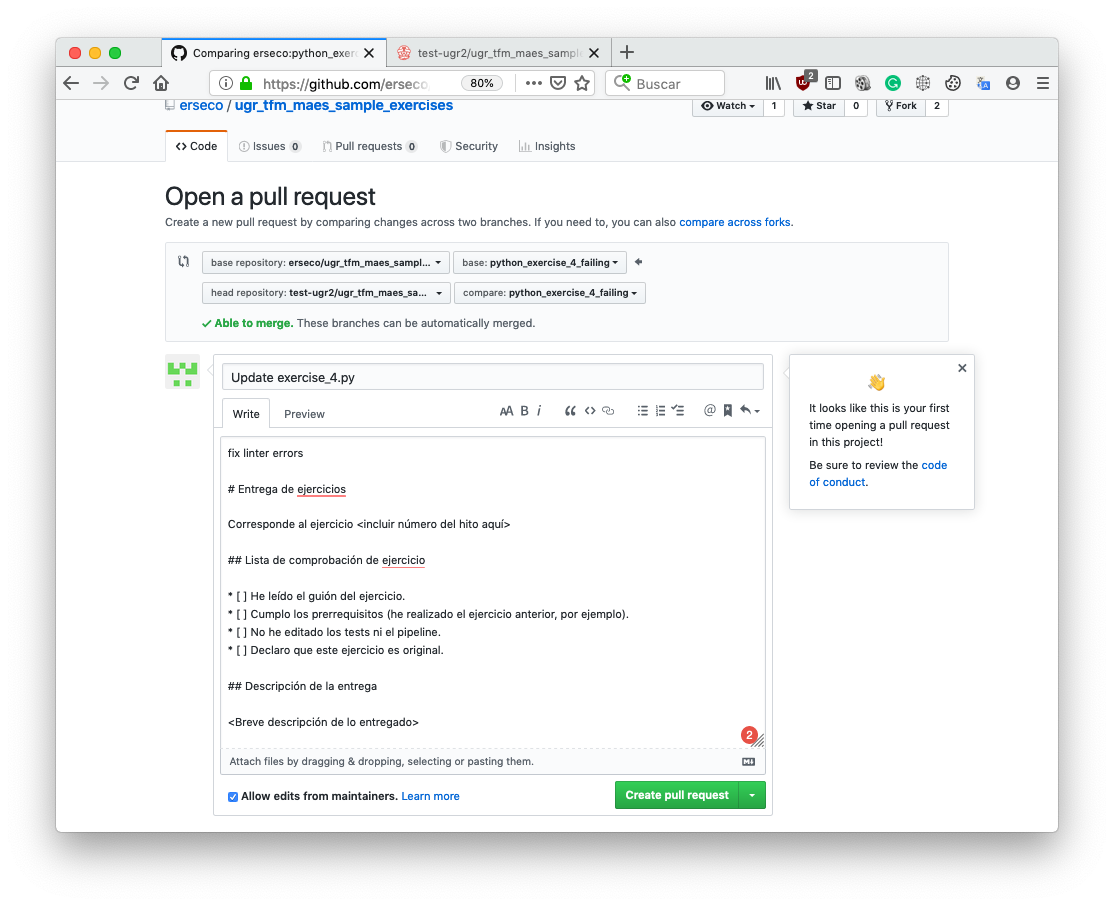
\includegraphics[width=1.0\textwidth]{../images/github_pr_create}
\caption{Plantilla de creación de Pull Request}
\label{fig:github_pr_create}
\end{figure}

Al crear el \textit{pull request} el alumno deberá verificar que no hay conflictos con el código base, si los hubiera deberá corregirlos manualmente. Tras esto se lanzarán los \textit{pipelines} del repositorio del alumno (se activan en cada envío) y el del repositorio del profesor, que se activa al crear el \textit{pull request} (figura \ref{fig:github_pr_view}) y al hacer cualquier envío adicional a la rama asociada al \textit{pull request}. Tras terminar el proceso de ejecución del \textit{pipeline} veremos si este ha dado un error (figura \ref{fig:travis_pipeline_failed}) o ha terminado de forma satisfactoria (figura \ref{fig:travis_pipeline_passed}) siendo esta última la imprescindible para proceder a corregir el ejercicio.

\begin{figure}[h!]
\centering
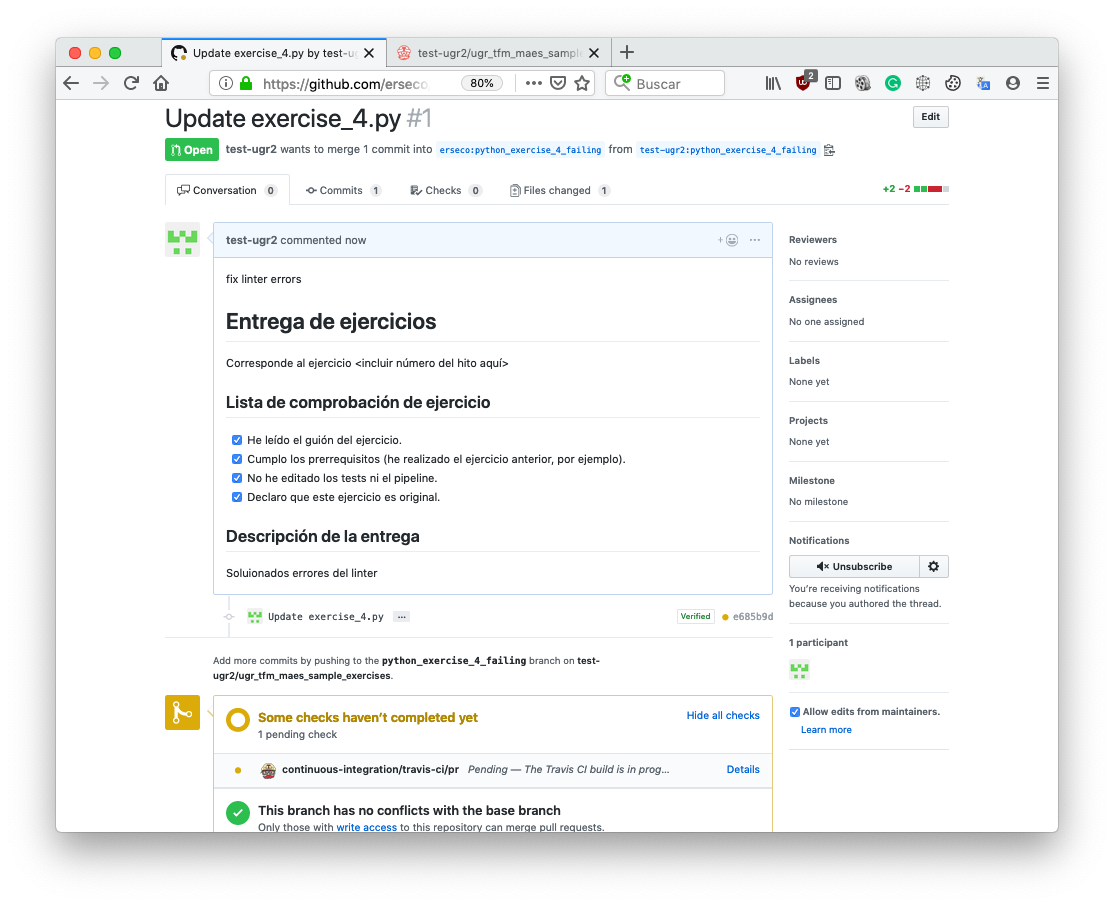
\includegraphics[width=1.0\textwidth]{../images/github_pr_view}
\caption{Vista de un Pull Request creado con el pipeline en ejecución}
\label{fig:github_pr_view}
\end{figure}

\begin{figure}[h!]
\centering
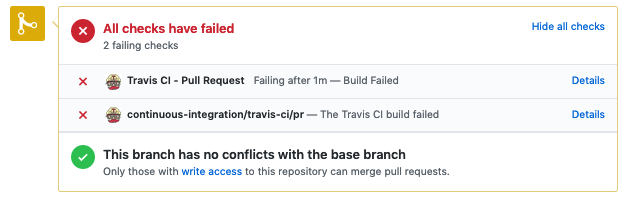
\includegraphics[width=1.0\textwidth]{../images/travis_pipeline_failed}
\caption{Detalle de un pipeline fallido}
\label{fig:travis_pipeline_failed}
\end{figure}

\begin{figure}[h!]
\centering
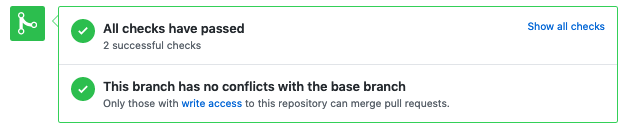
\includegraphics[width=1.0\textwidth]{../images/travis_pipeline_passed}
\caption{Detalle de un pipeline satisfactorio}
\label{fig:travis_pipeline_passed}
\end{figure}

\section{Evaluación}

Para la evaluación de los ejercicios nos basaremos en primer lugar en si han seguido los pasos indicados de forma correcta, realizando un ``Pull request'' e indicando lo realizado, luego comprobaremos si los ``pipelines'' han pasado de forma correcta y de forma adicional podemos entrar a valorar, como hemos mencionado anteriormente, el histórico de envíos a GitHub para ver si ha ido solucionando los problemas de forma adecuada y también valorando el tiempo dedicado. Esto no quiere decir que a más tiempo mayor calificación, pero si que sirve para hacernos una idea del esfuerzo que ha invertido el alumno para solucionar los ejercicios. Esto no quiere decir que también se pueda realizar una corrección ``manual'' de los ejercicios si fuera necesario.

\bigskip
Una utilidad muy útil de nuestro sistema es que podemos ver los cambios de forma visual con la pagina de diferencias, o \textit{diff} (figura \ref{fig:github_pr_diff}) lo que nos permite centrarnos en los cambios que ha realizado el alumno, además de detectar cualquier posible intento de modificación del código del \textit{pipeline} o de los tests de verificación, con esto nos podemos asegurar en la evaluación de que todo lo entregado por el alumno está realizado conforme al guión entregado.

\begin{figure}[h!]
\centering
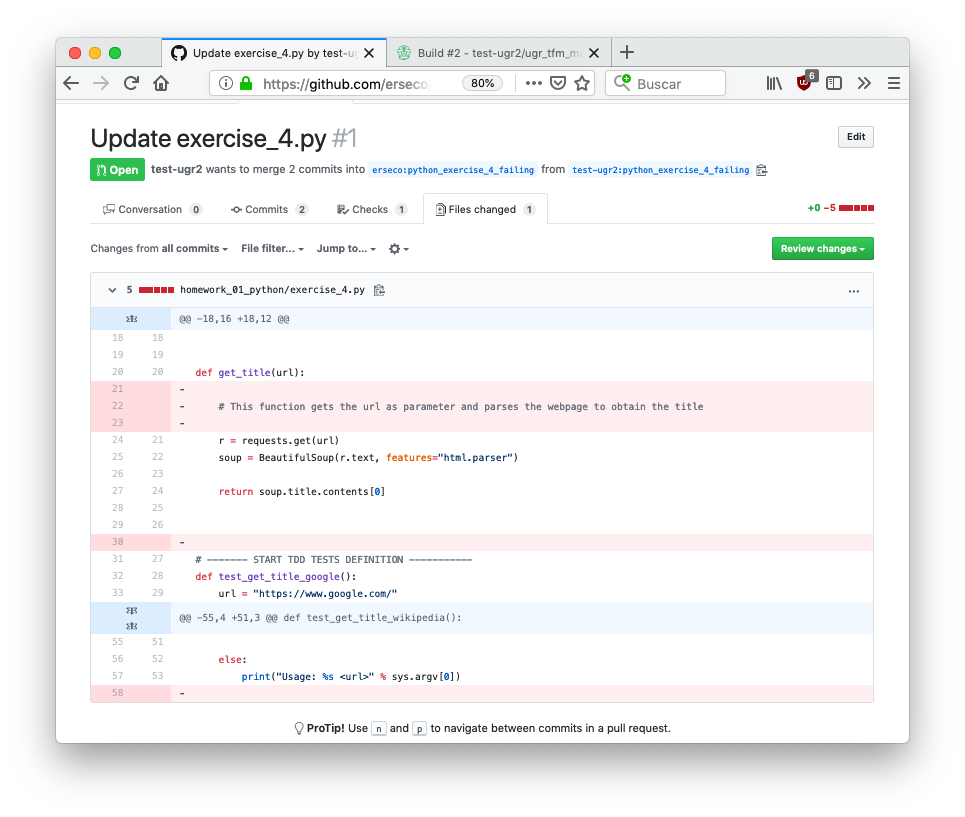
\includegraphics[width=1.0\textwidth]{../images/github_pr_diff}
\caption{Detalle de los cambios de código en un Pull Request}
\label{fig:github_pr_diff}
\end{figure}

% Falta mucho aquí acerca de la forma de trabajar: cómo plantear los ejercicios, cómo hacerlos con distintos objetivos y niveles, cómo se puede plantear la evaluación y calificación.... todo eso es parte de tu propuesta que puede ser un poco "independiente" de la propuesta tecnológica




\chapter{Propuesta Metodológica}

En este capítulo vamos a definir y a detallar los procesos que vamos a seguir para llevar a cabo la propuesta pedagógica definida en el capítulo anterior.

\section{Herramientas necesarias}

\subsection{Sistemas de control de versiones}

Lo primero que necesitaremos es enseñar a nuestros alumnos a utilizar un sistema de control de versiones, aunque existen varios sistemas (SVN, Mercurial, CVS), hoy en día estándar de facto es Git que además es software libre.

Para una administración más sencilla de nuestro código utilizaremos un cliente web como es GitHub, aunque existen otros como pueden ser GitLab o BitBucket.

\subsubsection {Git}

Git es un sistema de control de versiones distribuido que nos ayuda a llevar un seguimiento de los cambios en el código mientras desarrollamos. Se diseñó para su uso con código fuente pero se puede utilizar para llevar el seguimiento de los cambios en cualquier conjunto de archivos. Sus características incluyen la velocidad, la integridad de los datos y la compatibilidad con flujos de trabajo distribuidos y no lineales.

Git fue creado por Linus Torvalds en 2005 para el desarrollo del núcleo de Linux como alternativa al software BitKeeper que era un sistema de control de versiones propietario tras cambios en la licencia de este último.

Como con la mayoría de los sistemas de control de versiones distribuidos, y a diferencia de la mayoría de los sistemas cliente-servidor cada directorio de Git es un repositorio completo con un historial completo y capacidades de seguimiento de versiones completas, independiente del acceso a la red o a un servidor central.

Git es software libre y de código abierto distribuido bajo los términos de la Licencia Pública General GNU versión 2.

\subsubsection {GitHub}

GitHub es un servicio de alojamiento basado en web para el control de versiones a través de Git, fue adquirido por MicroSoft en 2018. Se utiliza sobre todo para código fuente aunque se puede utilizar para almacenar todo tipo de contenidos, incluso libros. Ofrece toda la funcionalidad de control de versiones distribuido y gestión de código fuente de Git, además de añadir sus propias características.

Proporciona control de acceso y varias funciones de colaboración como seguimiento de errores, \textit{pull requests}, gestión de tareas y \textit{wikis} para cada proyecto. Además cuenta con un sub-proyecto llamado GitHub Education que es ampliamente utilizado como herramientas para la formación de programadores (\cite{hernandez_integracion_2018}).


\section {Sistemas de integración continua (CI)}

\subsubsection {Travis-CI}

Travis CI es un servicio alojado de integración continua que se utiliza para construir y testear proyectos de software alojados en GitHub.

Los proyectos de código abierto pueden ser probados de forma gratuita a través del sitio \url{https://travis-ci.org}. En cambio los proyectos privados deben pagar para poder ser ejecutados a través del sitio \url{https://travis-ci.com}.

Gran parte de su código fuente es software libre y está disponible en GitHub.

\subsection{Lenguajes utilizados}

Al igual que no existe una única solución a un problema, existen multitud de lenguajes de programación, nosotros nos vamos a centrar en solamente cuatro de ellos ya que son los que cumplen con los contenidos de la mayoría de las asignaturas sobre informática, dichos lenguajes son Python, Ruby, C y HTML, aun así esta metodología es aplicable a otros lenguajes por lo que se podría utilizar para enseñar Java, Go, Haskell o Javascript:

\subsubsection{Python}

Python es un lenguaje de programación desarrollado por Guido van Rossum en 1991 cuya sintaxis favorece escribir código muy legible. Hoy en día es uno de los lenguajes de programación más utilizados en cursos de introducción a la programación ya que su sintaxis suele ser más sencilla, asemejándose al ``pseudocódigo''.

Según diversos índices (\cite{TIOBE2019}) y encuestas (\cite{stack_overflow_stack_2019}) Python es uno de los lenguajes con mayor proyección de futuro y que del que mas se ha incrementado su uso, sobre todo motivado por su sencillez a la hora de aprenderlo y a su potencia como lenguaje de análisis de datos habiendo prácticamente desbancando al lenguaje estadístico R.

\bigskip
Vamos a centrar nuestros ejercicios en la versión 3 de Python ya que la versión 2 actualmente solo recibe actualizaciones de seguridad y en enero de 2020 dejará de estar oficialmente soportada (\cite{python.org_pep_2018}).

\subsubsection{Ruby}

Ruby es un lenguaje de programación orientado a objetos creado por el programador japonés Yukihiro Matsumoto en 1995. Su orientación a objetos es denominada ``fuerte'' ya que todos los tipos de dato son a su vez un objeto.

\bigskip
Ruby empezó a ganar popularidad tras la publicación del framework de aplicaciones web Ruby On Rails (RoR) por parte de David Heinemeier Hansson en 2005 ya que el mismo simplificaba muchísimo el desarrollo siguiendo el patrón Modelo Vista Controlador (MVC).

\bigskip
Debido a su sencilla sintaxis y su fuerte orientación a objetos es ampliamente utilizado para enseñar las particularidades de dicho paradigma.

\subsubsection{C}

El lenguaje de programación C es un lenguaje de propósito general desarrollado por Dennis Ritchie en los Laboratorios Bell entre 1969 y 1972, es el lenguaje de programación más popular para crear software para sistemas embebidos y micro-controladores, aunque también se puede utilizar para crear aplicaciones.

\bigskip
Es un lenguaje tipado estáticamente (en tiempo de compilación) y considerad de de medio nivel ya que dispone de las estructuras típicas de los lenguajes de alto nivel pero permitiendo un control a muy bajo nivel. Los compiladores suelen ofrecer extensiones al lenguaje que posibilitan mezclar código en ensamblador con código C, acceder a memoria o controlar diferentes dispositivos.

\subsubsection{HTML}

El lenguaje de marcas de hipertexto o HTML por sus siglas en inglés, es un lenguaje de marcado para la elaboración de páginas web. La primera versión del lenguaje fue creada por Tim Berners-Lee en 1991 mientras trabajaba en el Centro Europeo de Investigaciones Nucleares (CERN) en Suiza. Actualmente sus especificaciones están a cargo del World Wide Web Consortium (W3C).

\bigskip
HTML no es un lenguaje de programación, es un lenguaje de marcado que sirve para definir documentos estandarizados.

\section {Herramientas de análisis de código}

También conocidos como ``linters''  son herramientas que analizan el código fuente para marcar errores de programación, \textit{bugs}, errores estilísticos y código sospechosos. Algunos son capaces incluso de calcular la complejidad ciclomática\footnote{Valor escalar que mide la complejidad lógica de un programa.} de un algoritmo. El término proviene de una antigua utilidad de Unix para análisis de código fuente en lenguaje C llamada ``lint''.

\bigskip
Existen \textit{linters} para prácticamente todos los lenguajes de programación, en nuestros ejemplos hemos utilizado los siguientes:

\subsection {Pycodestyle}

Pycodestyle es una herramienta para comprobar código fuente en el lenguaje Python contra las convenciones de estilo PEP8.

\bigskip
PEP8 es una guía de estilo de codificación para Python definida inicialmente por Guido van Rossum, creador del lenguaje Python y que está considerada como la estándar del lenguaje.

\subsection{Rubocop}

Es un analizar de código para el lenguaje Ruby que tiene opciones muy interesantes como el cálculo de la complejidad ciclomática y la auto-reparación de código fuente incorrecto.

\subsection{Cpplint}

Herramienta de código abierto desarrollada por Google, diseñada para garantizar que el código C y C++ se ajusta a las guías de estilo de codificación de la compañía.

\subsection {HTML Tidy}

Es una aplicación de consola que sirve para corregir código HTML no válido, detectar posibles errores de accesibilidad web y mejorar el diseño y el estilo de sangría del marcado resultante. Fue desarrollado en 2002 por el miembro del World Wide Web Consortium (W3C) Dave Raggett.

\section {Herramientas de verificación de código}

Las herramientas de verificación de código se utilizan para ejecutar los test TDD o BDD en nuestro código fuente. En nuestros ejercicios vamos a utilizar las siguientes  :

\subsection {Pytest}

Pytest es un framework de test unitarios para el lenguaje de programación Python que facilita la creación de pruebas sencillas y escalables. Las pruebas son expresivas y legibles y no se requiere código adicional.

\subsection {RSpec}

RSpec es una herramienta para realizar test BDD que sirve para probar código escrito en el lenguaje de programación Ruby.

\subsection{MinUnit}

MinUnit es un mini-framework para correr test unitarios en lenguaje C. Su código fuente se puede encontrar en \url{http://www.jera.com/techinfo/jtns/jtn002.html}. Es particularmente pequeño ya que consiste en un fichero de cabecera ``.h'' de tan solo 4 líneas de código.

\section{Metodología de aprendizaje}

Algunas de las herramientas necesarias para nuestro sistema de corrección requieren algo de formación previa, por lo que vamos a definir una metodología de aprendizaje para las mismas

\subsection{Aprendiendo a usar Git}

Como ya explicamos anteriormente Git es uno de los sistemas de control de versiones más utilizados en la actualidad. Es difícil encontrar hoy en día una empresa que se dedique a la programación de forma profesional que no la utilice. A pesar de ello no forma parte del currículo de los ciclos formativos de informática. De hecho, salvo contadas excepciones, tampoco se aprende su uso en los Grados en Ingeniería Informática. De ahí la ventaja de nuestro sistema, ya que vamos a aprovechar para enseñarles a utilizar una herramienta que van a usar de forma exhaustiva durante su futura carrera profesional.

\bigskip
Para aprender a utilizar Git nos vamos a basar en diversos manuales que enseñan a utilizarlo de una forma sencilla (\cite{popov_control_2012}) sin necesidad de tener conocimientos de programación. Como ya indicamos en la propuesta pedagógica vamos a definir unos contenidos comunes que son los siguientes:

\subsubsection{Introducción a Git}

En esta parte les explicaremos que es un sistema de control de versiones, que diferencias hay entre un sistema centralizado y uno distribuido. También les hablaremos de la motivación de por qué usarlos poniéndoles ejemplos de lo que seguramente ellos han utilizado hasta ahora que seguramente será duplicar los archivos en distintas carpetas. También les hablaremos un poco de la historia de Git.

\subsubsection{Creando una cuenta en GitHub}

Aquí les indicaremos como crear su primera cuenta en GitHub, para ello deberán acceder a la página web \url{https://github.com} y hacer clic en SignUp (figura \ref{fig:git1}).

\begin{figure}[H]
\centering
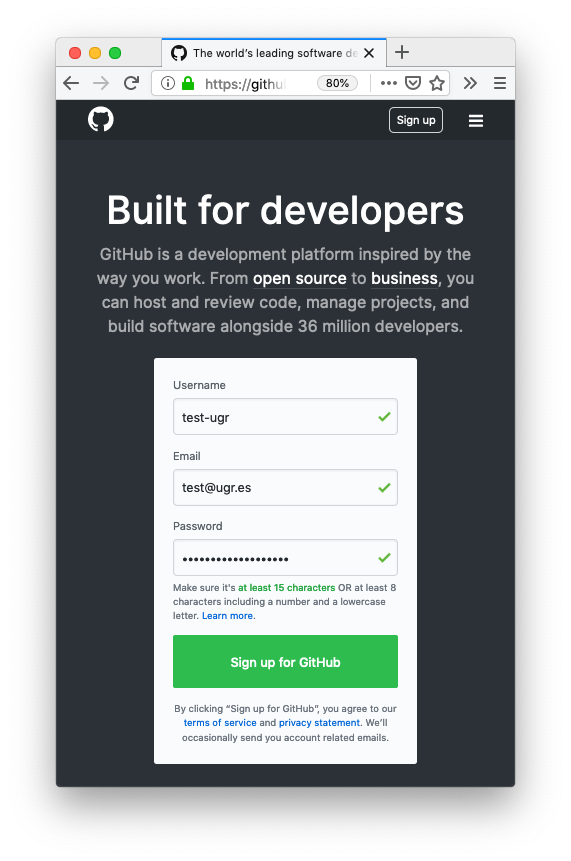
\includegraphics[width=1.0\textwidth]{../images/git1}
\caption{Pagina de registro de GitHub}
\label{fig:git1}
\end{figure}

\subsubsection{Creando nuestro primer repositorio}

Crear un repositorio en GitHub es muy intuitivo, solo tenemos que hacer clic en el botón New y rellenar los datos que nos solicita (figura \ref{fig:git2}). De igual forma podemos crear un repositorio de forma local en nuestro ordenador ejecutando el comando \texttt{git init}

\begin{figure}[H]
\centering
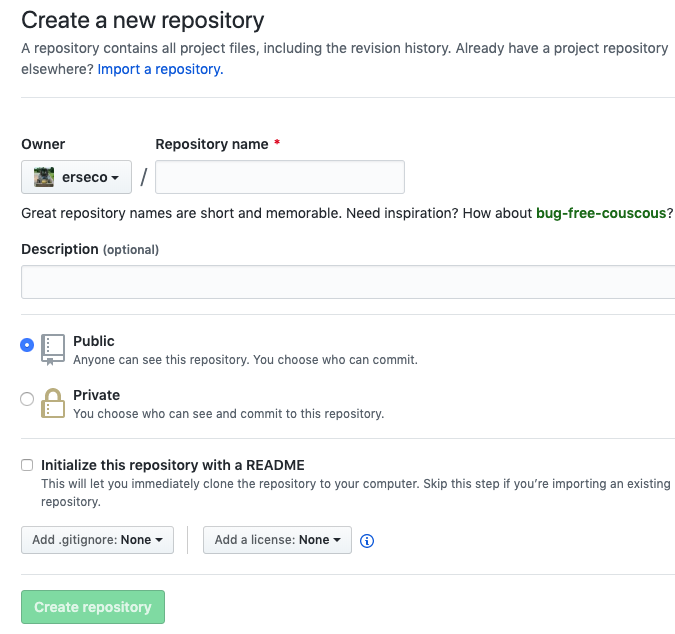
\includegraphics[width=1.0\textwidth]{../images/git2}
\caption{Ventana de creación de repositorio en GitHub}
\label{fig:git2}
\end{figure}

Para que los alumnos se familiaricen con el uso de GitHub editaremos el fichero \textcc{README.md} con el editor WYSIWYG\footnote{acrónimo de What You See Is What You Get (en español, "lo que ves es lo que obtienes").} integrado en la plataforma.

\subsubsection{Comandos básicos de Git}

Aquí podemos ver algunos de los comandos más habituales de Git, se puede encontrar la referencia completa en su documentación oficial en \url{https://git-scm.com/doc}.

\begin{itemize}
  \item \textbf{git clone}: Clona un repositorio
  \item \textbf{git status}: Nos dice el estado de un repositorio
  \item \textbf{git commit}: Nos permite guardar los cambios en una rama
  \item \textbf{git checkout}: Nos permite cambiar de rama
  \item \textbf{git branch}: Nos permite crear y listar ramas
  \item \textbf{git push}: Permite enviar el código a un repositorio remoto
  \item \textbf{git pull}: Permite obtener el código desde un repositorio remoto
\end{itemize}

Para que los alumnos se familiaricen con el uso de estos comandos vamos a pedirle que hagan cambios en los archivos de la carpeta \textcc{homework_00_markdown} con su editor y hagan un \textit{commit} y un \textit{push} con el código fuente.

\subsubsection{Creando nuestro primer Fork}

Una bifurcación, o fork en inglés, es el término que se utiliza para indicar una ramificación de un trabajo. Básicamente significa que vamos a copiar un proyecto y crear uno nuevo haciéndole modificaciones. La capacidad de crear bifurcaciones de código de forma sencilla es una de las características que han ayudado a la plataforma GitHub llegar a ser el sitio de referencia para albergar proyectos de software libre.

\bigskip
Para crear un fork en GitHub de cualquier proyecto simplemente tenemos que hacer click en el botón situado a la derecha de cada proyecto (figura \ref{fig:git_fork}). Una cosa a tener en cuenta a la hora de hacer un Fork de un proyecto es la licencia bajo la que esté dicho código, el cual suele venir indicado en el fichero LICENSE, no todas las licencias permiten la libre distribución de proyectos derivados.

\begin{figure}[H]
\centering

\includegraphics[width=1.0\textwidth]{../images/git_fork}
\caption{Detalle del botón de Fork en GitHub}
\label{fig:git_fork}
\end{figure}

\subsubsection{Creando un Pull-Request}

Las contribuciones a un repositorio de código fuente que utiliza un sistema de control de versiones distribuido se realizan comúnmente por medio de un ``pull request''. El colaborador solicita que el encargado del proyecto haga un ``pull'' con los cambios en el código fuente, de ahí el nombre. El mantenedor puede revisar el conjunto de cambios, discutir modificaciones potenciales o mezclar el código.

Dependiendo del flujo de trabajo establecido el código puede ser probado antes de ser incluido en la versión oficial. Algunos proyectos ejecutan un conjunto de pruebas automatizadas en cada solicitud de extracción, utilizando una herramienta de integración continua como Travis CI, y el revisor verifica que cualquier código nuevo tenga la cobertura de pruebas adecuada.

Para hacer un ``Pull request'' haremos clic en el botón ``New pull request'' y seleccionando que ramas queremos fusionar (figura \ref{fig:git_pr}).

\begin{figure}[H]
\centering
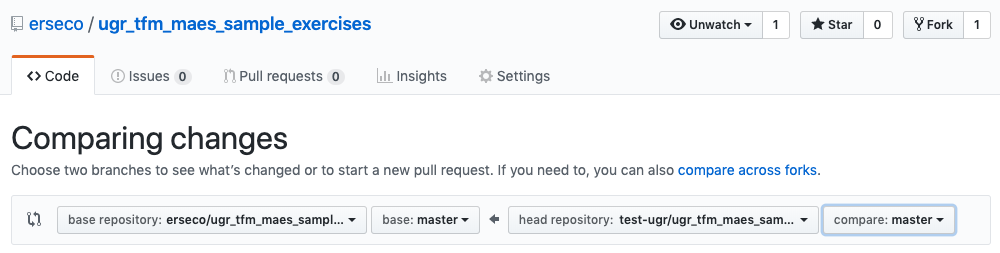
\includegraphics[width=1.0\textwidth]{../images/git_pr}
\caption{Detalle de creación de un Pull Request en GitHub}
\label{fig:git_pr}
\end{figure}

\subsubsection{Sistemas de integración continua (CI)}

Un sistema de integración continua suele consistir en una plataforma que ejecuta una serie de pasos con cada ``Push'' que realizamos a nuestro sistema de control de versiones. A esta serie de pasos se le suele denominar ``pipeline'' y suele contener pasos habituales como pueden ser la compilación, la ejecución de validaciones sintácticas y estilísticas de código (\textit{linter}) y la ejecución de los diferentes test para comprobar que efectivamente el código funciona.

\bigskip
Como ya hemos indicado, para nuestra metodología vamos a utilizar ``Travis CI'' aunque la forma de funcionar es muy similar en casi todas las plataformas. Para crear una cuenta en ``Travis CI'' iremos a la url \url{https://travis-ci.org} y haremos click en el botón ``Sign-Up'' (figura \ref{fig:travis_signup})).

\begin{figure}[H]
\centering
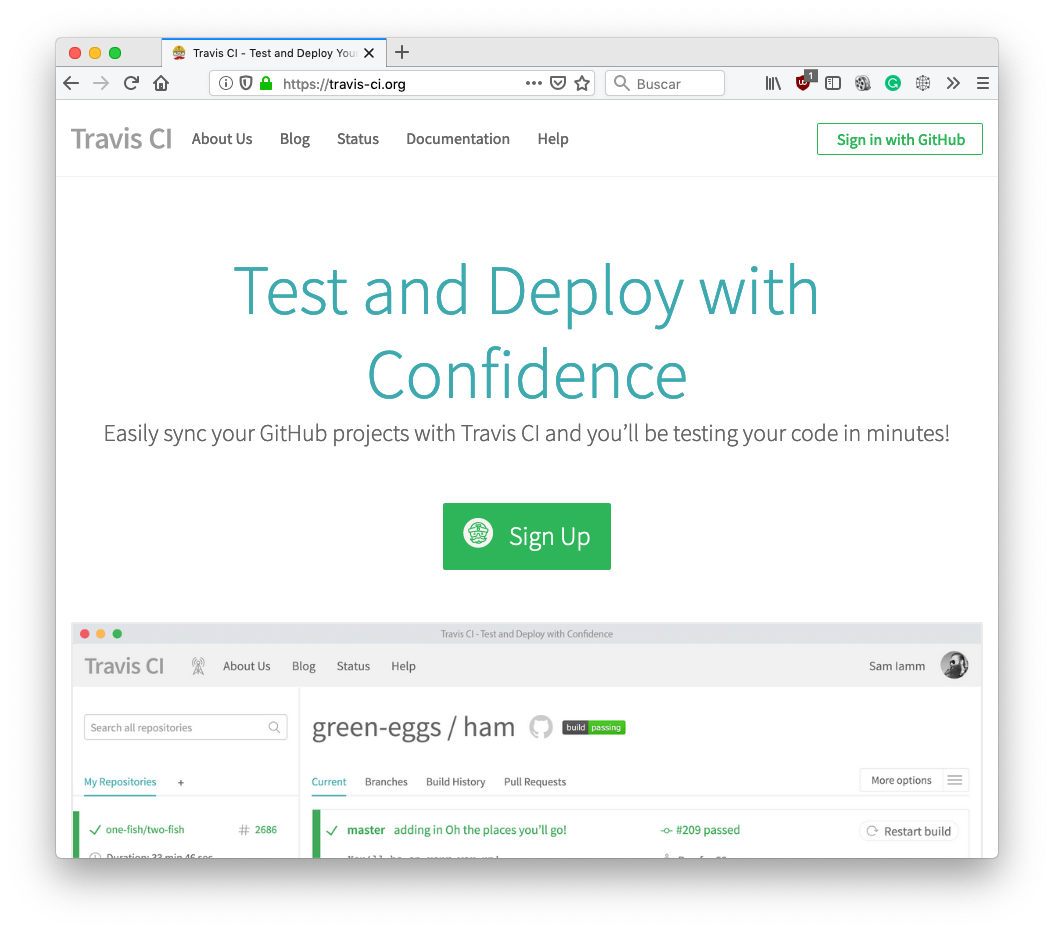
\includegraphics[width=1.0\textwidth]{../images/travis_signup}
\caption{Detalle de creación de una cuenta en Travis CI}
\label{fig:travis_signup}
\end{figure}

Una vez tengamos nuestra cuenta tenemos que activar en cuales de nuestra lista de repositorios queremos activar el servicio. Para ellos solo debemos hacer click en el interruptor hasta que quede de color verde (figura \ref{fig:travis_enable}).

\begin{figure}[H]
\centering
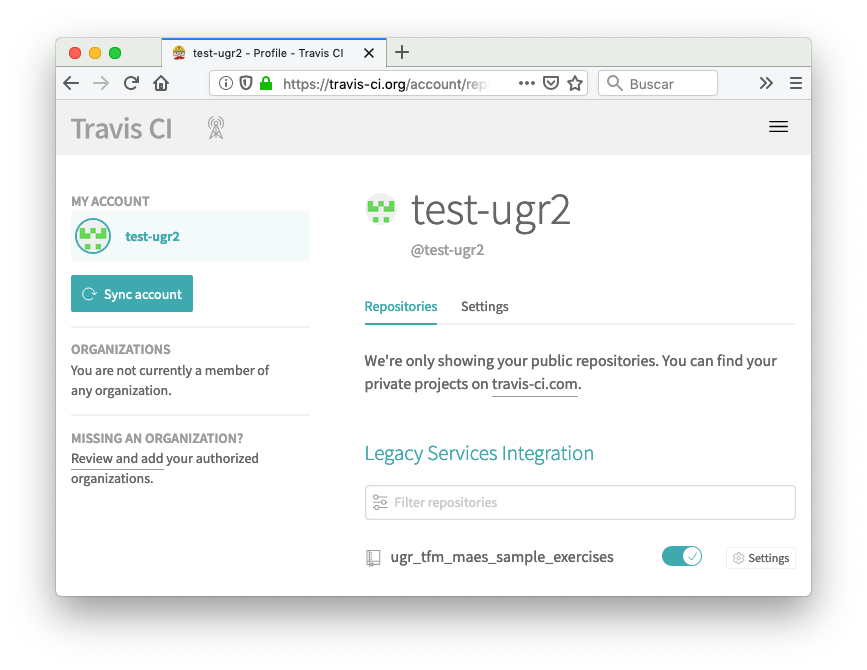
\includegraphics[width=1.0\textwidth]{../images/travis_enable}
\caption{Detalle de activación de un repositorio en Travis CI}
\label{fig:travis_enable}
\end{figure}

Una vez activado, con cada \texttt{git push} se ejecutará el ``pipeline'' definido en el fichero \texttt{.travis.yml}, en nuestro repositorio de ejemplo se puede obtener uno configurado para ejecutar los diferentes ejemplos realizados para mostrar el funcionamiento de la metodología.

\subsection{Introducción a la programación}

Una vez los alumnos han aprendido los comandos básicos de Git y se han dado de alta en GitHub es hora de enseñarles algunos conceptos básicos de programación.

\subsubsection{Conceptos básicos de programación}

Todos los lenguajes de programación comparten algunos elementos básicos que funcionan y se usan de forma diferente en cada lenguaje, pero que cumplen el mismo objetivo. Esos elementos son:

\begin{itemize}
  \item Tipos de datos: Enteros, Decimales, Caracteres, Cadenas de texto, etc...
  \item Variables: donde almacenar los datos.
  \item Control de flujo: los ``if''
  \item Bucles: los conocidos ``loops'', ``for'' y ``while''
  \item Funciones
  \item Entra y Salida: pintando en pantalla.
\end{itemize}

Hay que remarcar que estamos explicando los conceptos básicos de programación, por eso esto no incluye ni estructuras de datos, ni orientación a objetos ni recursividad, realmente eso lo aprenderán en ejercicios adicionales.

\subsubsection{Nuestro primer ``Hola Mundo''}

Un ``Hola mundo'' es un programa cuya única finalidad es escribir la frase ``Hola mundo!''. Este programa se usa como introducción en la mayoría de lenguajes de programación siendo el primer ejercicio típico, y se considera fundamental desde el punto de vista didáctico. Una implementación de dicho programa se puede encontrar para prácticamente todos los lenguajes de programación existentes.

\bigskip
En nuestra metodología animamos a los profesores a enseñar un primer ejemplo del lenguaje a impartir usando un ``Hola Mundo'' para que los alumnos se familiaricen con el lenguaje. En nuestros ejercicios de ejemplo vamos a incorporar el hola mundo como primer ejercicio de programación.

\subsubsection{Guías de estilo}

En esta sección les enseñaremos la guía de estilo que vamos a seguir. Aunque es algo que se suele obviar en cursos de programación, a la hora de escribir código de calidad es importante seguir una guía de estilo, además de crear buenas prácticas de programación. Les explicaremos lo importante que es comentar correctamente y se utilizará a poder ser una guía de estilo estandarizada para el lenguaje que vayamos a impartir.

\bigskip
Si el lenguaje que vamos a impartir no tuviera guía de estilo estandarizada, o si el profesor lo estima didáctico se podría consensuar con los alumnos el tipo de estilo que se va a seguir. Este caso es aplicable al uso de comillas simples '' o dobles "" pues no hay un consenso sobre cuales se deben usar, igual pasa con la indentación con espacios o con tabuladores.

\subsubsection{Introducción al TDD}

Aquí les explicaremos en consiste el TDD, que como ya hemos visto es escribir la prueba, escribir el código y una vez funcione refactorizar. En nuestro caso concreto les vamos a dar nosotros realizadas las pruebas TDD, pero les podremos animar a que realicen pruebas adicionales.

\subsubsection{Ejercicios de ejemplo}

En el repositorio \url{https://github.com/erseco/ugr_tfm_maes_sample_exercises} hemos definido una serie de ejercicios así como sus correcciones, dichos ejercicios se han incorporado en la sección de Anexos.

\subsection{Usando la integración continua para aprender}

Una vez hemos visto como usar Git y los conceptos básicos de programación vamos a ver algunos de los errores con los que se pueden encontrar los alumnos, como pueden usar el sistema de integración continua para detectarlos ellos mismos y como corregirlos (figura \ref{fig:linter_error_python}).

\begin{figure}[H]
\centering
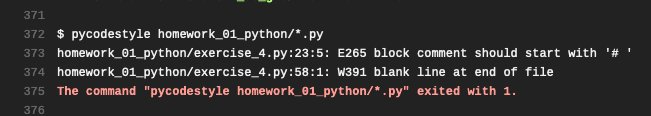
\includegraphics[width=1.0\textwidth]{../images/linter_error_python}
\caption{Detalle de un error de linter python en un pipeline}
\label{fig:linter_error_python}
\end{figure}



\chapter{Conclusiones}

Una vez realizada tanto la propuesta técnica como la propuesta pedagógica podemos ver como a pesar de sus inconvenientes los sistema de autocorrección nos proveen de diversas ventajas.

\section{Ventajas}

Al estar la corrección basada en los tests definidos por ele profesor la solución es agnóstica del lenguaje, el mismo método nos puede servir para enseñar cualquier lenguaje de programación o incluso un paradigma concreto.

Podemos usar el mismo método tanto para cursos de iniciación como para cursos mucho más complejos.

Como ya hemos visto en la propuesta pedagógica podemos definir las pautas pedagógicas de la corrección.

Tal y como dice (REFERENCIA ESTUDIO), mejora la interacción con el alumno.

Al guardarse un registro de todo lo que se envía al repositorio de código junto al resultado de su compilación, el profesor puede tener métricas muy detalladas de los errores cometidos por cada alumno, ver su evolución e incluso el tiempo dedicado.

Es fácil detectar el plagio.

El profesor puede ir haciendo futuras modificaciones sobre los ejercicios para incidir en los temas en los que los alumnos tengan mayor dificultad.


\section{Inconvenientes}

El profesor tiene que estar atento para evitar el plagio, asimismo debe de cambiar regularmente los ejercicios ya que al estar disponibles en Internet una simple búsqueda les permitiría a los alumnos obtener la resolución de los ejercicios de cursos anteriores.

La curva de trabajo para el profesor es mas pronunciada al principio pues debe de preparar una gran variedad de ejercicios y test antes del comienzo de las clases.




\chapter{Anexos}

\section{Código fuente}

\subsection{Pipeline para Travis-CI}

\begin{lstlisting}[language=yaml,caption={.travis.yml},captionpos=b]
---
dist: xenial

before_install:
  - pyenv global system 3.6.7
  - sudo apt-get update
  - sudo apt-get install -y tidy cppcheck
install:
  - pip3 install pytest pycodestyle requests beautifulsoup4
  - gem install rspec rubocop mdl

script:
  - echo "Testing that we have all the requirements"
  - mdl --version
  - python3 --version
  - ruby --version
  - gcc --version
  - tidy --version

  - mdl homework_00_git/

  - pycodestyle homework_01_python/*.py
  - pytest --verbose homework_01_python/*.py

  - rubocop homework_02_ruby
  - rspec homework_02_ruby

  - cppcheck --verbose --error-exitcode=2 homework_03_c/*.c
  - make -C homework_03_c tests

  - tidy -quiet -errors homework_04_html/*.html
\end{lstlisting}

\subsection{Ejercicios Git/Markdown}
\begin{lstlisting}[language=markdown,caption={exercise\_01.md},captionpos=b]
# Hello world
\end{lstlisting}

\begin{lstlisting}[language=markdown,caption={exercise\_02.md},captionpos=b]
#h1 Heading

## h2 Heading

### h3 Heading

#### h4 Heading

##### h5 Heading

## Horizontal Rule
___


## Emphasis

Text **This is bold text**

Text *This is italic text*

Text _This is italic text_

Text ~~Strikethrough~~

## Lists

- Create a list by starting a `-`
- Very easy!

## Code

```
Sample text here...
```

## Tables

| name   | description |
| ------ | ----------- |
| name1  | description1. |
| name2  | description2. |
| name3  | description3. |

## Links

[link text](http://www.google.es)

[link with title](http://www.google.es/ "title text!")
\end{lstlisting}

\subsection{Ejercicios Python}
\begin{lstlisting}[language=python,caption={exercise\_1.py},captionpos=b]
#!/usr/bin/env python3

# Question:
# Write a program that prints "Hello world!"
#
# Hints:
# Use the python print() built-infunction


print('Hola mundo!')
\end{lstlisting}

\begin{lstlisting}[language=python,caption={exercise\_2.py},captionpos=b]
#!/usr/bin/env python3

# Question:
# Write a function called add() which can compute and returns the summ of two
# given numbers.
#
# Suppose the following parameters are supplied to the program:
# 8 8
# Then, the output should be:
# 16

import sys


def add(x, y):
    return x + y


# ------- START TDD TESTS DEFINITION -----------
def test_add_8_8():
    assert add(8, 8) == 16


def test_add_4_5():
    assert add(4, 5) == 9
# ------- END TDD TESTS DEFINITION -------------


# Program entrypoint
if __name__ == "__main__":

    if len(sys.argv) == 3:

        number1 = int(sys.argv[1])
        number2 = int(sys.argv[2])
        result = add(number1, number2)
        print(result)

    else:
        print("Usage: %s <number1> <number2>" % sys.argv[0])
\end{lstlisting}

\begin{lstlisting}[language=python,caption={exercise\_3.py},captionpos=b]
#!/usr/bin/env python3

# Question:
# Write a function called get_factorial() which can compute and returns the
# factorial of a given number.
#
# Suppose the following parameter is supplied to the program:
# 8
# Then, the output should be:
# 40320
#
# Hints:
# You can't use the `math` module.

import sys


def get_factorial(number):
    if number == 0:
        return 1
    return number * get_factorial(number - 1)


# ------- START TDD TESTS DEFINITION -----------
def test_get_factorial_8():
    import math
    assert math.factorial(8) == get_factorial(8)


def test_get_factorial_3():
    import math
    assert math.factorial(3) == get_factorial(3)


def test_get_factorial_25():
    import math
    assert math.factorial(25) == get_factorial(25)
# ------- END TDD TESTS DEFINITION -------------


# Program entrypoint
if __name__ == "__main__":

    if len(sys.argv) == 2:
        number = int(sys.argv[1])
        result = get_factorial(number)
        print(result)

    else:
        print("Usage: %s <number>" % sys.argv[0])
\end{lstlisting}

\begin{lstlisting}[language=python,caption={exercise\_4.py},captionpos=b]
#!/usr/bin/env python3

# Question:
# Write a function that get the content of the <title> tag of a given url
#
# Suppose the following parameter is supplied to the program:
# https://www.google.es
# Then, the output should be:
# Google
#
# Hints:
# Use the requests module to read the web content
# Use the BeautifulSoup to process the HTML

import sys
import requests
from bs4 import BeautifulSoup


def get_title(url):

    r = requests.get(url)
    soup = BeautifulSoup(r.text, features="html.parser")

    return soup.title.contents[0]


# ------- START TDD TESTS DEFINITION -----------
def test_get_title_google():
    url = "https://www.google.com/"
    assert get_title(url) == "Google"


def test_get_title_alhambra():
    url = "http://www.alhambra-patronato.es/"
    assert get_title(url) == "Patronato de la Alhambra y Generalife"


def test_get_title_wikipedia():
    url = "https://en.wikipedia.org/wiki/Main_Page"
    assert get_title(url) == "Wikipedia, the free encyclopedia"
# ------- END TDD TESTS DEFINITION -------------


# Program entrypoint
if __name__ == "__main__":

    if len(sys.argv) == 2:
        url = sys.argv[1]
        result = get_title(url)
        print(result)

    else:
        print("Usage: %s <url>" % sys.argv[0])
\end{lstlisting}

\begin{lstlisting}[language=python,caption={exercise\_5.py},captionpos=b]
#!/usr/bin/env python3

# Question:
# Write a funciton that works like a "Rock-Paper-Scissors" game, remember the
# rules:
# - Rock beats scissors
# - Scissors beats paper
# - Paper beats rock
#
# The result should be:
# - It's a tie!
# - Rock wins!
# - Scissors win!
# - Paper wins!
# - Invalid input!
#
# Suppose the following parameter is supplied to the program:
# rock scissors
# Then, the output should be:
# Rock wins!


def play_game(option1, option2):

    if option1 == option2:
        return("It's a tie!")
    elif option1 == 'rock':
        if option2 == 'scissors':
            return("Rock wins!")
        else:
            return("Paper wins!")
    elif option1 == 'scissors':
        if option2 == 'paper':
            return("Scissors win!")
        else:
            return("Rock wins!")
    elif option1 == 'paper':
        if option2 == 'rock':
            return("Paper wins!")
        else:
            return("Scissors win!")
    else:
        return("Invalid input!")


# ------- START TDD TESTS DEFINITION -----------
def test_play_game_rock_scissors():
    assert play_game("rock", "scissors") == "Rock wins!"


def test_play_game_scissors_scissors():
    assert play_game("scissors", "scissors") == "It's a tie!"


def test_play_game_paper_rock():
    assert play_game("paper", "rock") == "Paper wins!"


def test_play_game_scissors_paper():
    assert play_game("scissors", "paper") == "Scissors win!"


def test_play_game_invalid_paper():
    assert play_game("invalid", "paper") == "Invalid input!"
# ------- END TDD TESTS DEFINITION -------------


# Program entrypoint
if __name__ == "__main__":

    if len(sys.argv) == 3:

        option1 = sys.argv[1]
        option2 = sys.argv[2]
        result = play_game(option1, option2)
        print(result)

    else:
        print("Usage: %s <option1> <option2>" % sys.argv[0])
\end{lstlisting}

\subsection{Ejercicios Ruby}
\begin{lstlisting}[language=ruby,caption={exercise\_1.rb},captionpos=b]
#!/usr/bin/env ruby
# frozen_string_literal: true

# Question:
# Write a program that prints "Hello world!"
#
# Hints:
# Use the ruby puts directive

puts 'Hello world!'
\end{lstlisting}

\begin{lstlisting}[language=ruby,caption={exercise\_2.rb},captionpos=b]
#!/usr/bin/env ruby
# frozen_string_literal: true

# Question:
# Write a function called add() which can compute and returns the summ of two
# given numbers.
#
# Suppose the following parameters are supplied to the program:
# 8 8
# Then, the output should be:
# 16

def add(number1, number2)
  number1 + number2
end

# Program entrypoint
if $PROGRAM_NAME == __FILE__
  if ARGV.length == 2

    number1 = ARGV[0].to_i
    number2 = ARGV[1].to_i
    result = add(number1, number2)
    puts result
  else
    puts "Usage: #{$PROGRAM_NAME} <number1> <number2>"
  end
end
\end{lstlisting}

\begin{lstlisting}[language=ruby,caption={exercise\_2\_spec.rb},captionpos=b]
# frozen_string_literal: true

require_relative '../exercise_2'

# ------- START TDD TESTS DEFINITION -----------
describe add(0, 0) do
  it 'returns 16 when passed 8 8' do
    expect(add(8, 8)).to eq 16
  end

  it 'returns 9 when passed 4 5' do
    expect(add(4, 5)).to eq 9
  end
end
# ------- END TDD TESTS DEFINITION -------------
\end{lstlisting}

\begin{lstlisting}[language=ruby,caption={exercise\_3.rb},captionpos=b]
#!/usr/bin/env ruby
# frozen_string_literal: true

# Question
# Write a function called get_factorial() which can compute and returns the
# factorial of a given number.
#
# Suppose the following parameter is supplied to the program
# 8
# Then, the output should be
# 40320
#
# Hints:
# You can't use the `math` module.

def get_factorial(number)
  return 1 if number.zero?

  number * get_factorial(number - 1)
end

# Program entrypoint
if $PROGRAM_NAME == __FILE__

  if ARGV.length == 1
    number = ARGV[0].to_i
    result = get_factorial(number)
    puts result
  else
    puts "Usage: #{$PROGRAM_NAME} <number>"
  end
end
\end{lstlisting}

\begin{lstlisting}[language=ruby,caption={exercise\_3\_spec.rb},captionpos=b]
# frozen_string_literal: true

require_relative '../exercise_3'

# ------- START TDD TESTS DEFINITION -----------
describe get_factorial(0) do
  it 'returns 40320 when passed 8' do
    expect(get_factorial(8)).to eq 40_320
  end

  it 'returns 6 when passed 3' do
    expect(get_factorial(3)).to eq 6
  end
  it 'returns 15511210043330985984000000 when passed 3' do
    expect(get_factorial(25)).to eq 15_511_210_043_330_985_984_000_000
  end
end
# ------- END TDD TESTS DEFINITION -------------
\end{lstlisting}

\begin{lstlisting}[language=ruby,caption={exercise\_4.rb},captionpos=b]
#!/usr/bin/env ruby

# Question:
# Write a function that get the content of the <title> tag of a given url
#
# Suppose the following parameter is supplied to the program:
# https://www.google.es
# Then, the output should be:
# Google
#
# Hints:
# Use the open-uri module to read the web content
# Use a regular expression to process the HTML
require "open-uri"

def get_title(url)
    open(url) do |f|
        str = f.read
        str.scan(/<title>(.*?)<\/title>/)
    end
end

# Program entrypoint
if __FILE__ == $PROGRAM_NAME

    if ARGV.length == 1
        url = ARGV[0]
        result = get_title(url)
        puts result

    else
        puts "Usage: #{$PROGRAM_NAME} <url>"
    end
end
\end{lstlisting}

\begin{lstlisting}[language=ruby,caption={exercise\_4\_spec.rb},captionpos=b]
# frozen_string_literal: true

require_relative '../exercise_4'

# ------- START TDD TESTS DEFINITION -----------
#  RSpec don't allow to connect to external websites, so we should mock the petition
describe get_factorial(0) do
    it 'returns "Google" when passed "https//www.google.com/"' do
      expect(get_title('https//www.google.com/')).to eq 'Google'
    end
    it 'returns "Patronato de la Alhambra y Generalife" when passed "http//www.alhambra-patronato.es/"' do
      expect(get_title('http//www.alhambra-patronato.es/')).to eq 'Patronato de la Alhambra y Generalife'
    end
    it 'returns "Wikipedia, the free encyclopedia" when passed "https//en.wikipedia.org/wiki/Main_Page"' do
      expect(get_title('https//en.wikipedia.org/wiki/Main_Page')).to eq 'Wikipedia, the free encyclopedia'
    end
end
# ------- END TDD TESTS DEFINITION -------------
\end{lstlisting}

\begin{lstlisting}[language=ruby,caption={exercise\_5.rb},captionpos=b]
#!/usr/bin/env ruby
# frozen_string_literal: true

# Question:
# Write a funciton that works like a "Rock-Paper-Scissors" game, remember the
# rules:
# - Rock beats scissors
# - Scissors beats paper
# - Paper beats rock
#
# The result should be:
# - It's a tie!
# - Rock wins!
# - Scissors win!
# - Paper wins!
# - Invalid input!
#
# Suppose the following parameter is supplied to the program:
# rock scissors
# Then, the output should be:
# Rock wins!

def play_game(option1, option2)
  if option1 == option2
    "It's a tie!"
  elsif option1 == 'rock'
    if option2 == 'scissors'
      'Rock wins!'
    else
      'Paper wins!'
    end
  elsif option1 == 'scissors'
    if option2 == 'paper'
      'Scissors win!'
    else
      'Rock wins!'
    end
  elsif option1 == 'paper'
    if option2 == 'rock'
      'Paper wins!'
    else
      'Scissors win!'
    end
  else
    'Invalid input!'
  end
end

# Program entrypoint
if $PROGRAM_NAME == __FILE__

  if ARGV.length == 2

    option1 = ARGV[0]
    option2 = ARGV[1]
    result = play_game(option1, option2)
    puts result

  else
    puts "Usage: #{$PROGRAM_NAME} <option1> <option2>"
  end
end
\end{lstlisting}

\begin{lstlisting}[language=ruby,caption={exercise\_5\_spec.rb},captionpos=b]
# frozen_string_literal: true

require_relative '../exercise_5'

# ------- START TDD TESTS DEFINITION -----------
describe play_game('', '') do
  it 'returns "Rock wins!" when passed "rock" "scissors"' do
    expect(play_game('rock', 'scissors')).to eq 'Rock wins!'
  end

  it 'returns "Its a tie!" when passed "scissors" "scissors"' do
    expect(play_game('scissors', 'scissors')).to eq "It's a tie!"
  end

  it 'returns "Paper wins!" when passed "paper" "rock"' do
    expect(play_game('paper', 'rock')).to eq 'Paper wins!'
  end

  it 'returns "Scissors win!" when passed ("scissors" "paper"' do
    expect(play_game('scissors', 'paper')).to eq 'Scissors win!'
  end

  it 'returns "Invalid input!" when passed "invalid" "paper"' do
    expect(play_game('invalid', 'paper')).to eq 'Invalid input!'
  end
end
# ------- END TDD TESTS DEFINITION -------------
\end{lstlisting}

\subsection{Ejercicios C}
\begin{lstlisting}[language=c,caption={Makefile},captionpos=b]
SRCS = $(wildcard *.c)
PROGS = $(patsubst %.c,%,$(SRCS))

all: $(PROGS)

%: %.c
  gcc $(CFLAGS) -o $@ $<

tests: test_2 test_3 test_5 clean

test_2:
  @gcc $(CFLAGS) -Wl, -e_main_tests -o exercise_2 exercise_2.c
  @./exercise_2

test_3:
  @gcc $(CFLAGS) -Wl, -e_main_tests -o exercise_3 exercise_3.c
  @./exercise_3

test_5:
  @gcc $(CFLAGS) -Wl, -e_main_tests -o exercise_5 exercise_5.c
  @./exercise_5

clean:
  @rm -f $(PROGS)
\end{lstlisting}

\begin{lstlisting}[language=c,caption={minunit.h},captionpos=b]
 /* file: minunit.h */
 #define mu_assert(message, test) do { if (!(test)) return message; } while (0)
 #define mu_run_test(test) do { char *message = test(); tests_run++; \
                                if (message) return message; } while (0)
int tests_run;

char * all_tests();

// This function acts as entrypoint for TDD
int main_tests(int argc, char **argv) {
     char *result = all_tests();
     if (result != 0) {
         printf("%s\n", result);
     }
     else {
         printf("ALL TESTS PASSED on %s\n", argv[0]);
     }
     printf("Tests run: %d\n", tests_run);

     return result != 0;
}
\end{lstlisting}

\begin{lstlisting}[language=c,caption={exercise\_1.c},captionpos=b]
/*
# Question:
# Write a program that prints "Hello world!"
#
# Hints:
# Use the c printf() built-infunction
*/

#include <stdio.h>

int main(void)
{
    printf("Hello world!\n");
    return 0;
}
\end{lstlisting}

\begin{lstlisting}[language=c,caption={exercise\_2.c},captionpos=b]
/*
# Question:
# Write a function called add() which can compute and returns the summ of two
# given numbers.
#
# Suppose the following parameters are supplied to the program:
# 8 8
# Then, the output should be:
# 16
*/

#include <stdio.h> //printf, scanf
#include <stdlib.h> //atoi, strtol
#include "minunit.h"

int add(int x, int y) {
    return x + y;
}

// ------- START TDD TESTS DEFINITION -----------
char * test_add_8_8(){
    mu_assert("error", add(8, 8) == 16);
    return 0;
}

char * test_add_4_5() {
    mu_assert("error", add(4, 5) == 9);
    return 0;
}

char * all_tests() {
     mu_run_test(test_add_8_8);
     mu_run_test(test_add_4_5);
     return 0;
 }
// ------- END TDD TESTS DEFINITION -------------

// Program entrypoint
int main(int argc, char **argv)
{

    if (argc == 3) {

        int number1 = atoi(argv[1]);
        int number2 = atoi(argv[2]);
        int result = add(number1, number2);
        printf("%d\n", result);

    } else {
        printf("Usage: %s <number1> <number2>\n", argv[0]);
    }

    return 0;
}
\end{lstlisting}

\begin{lstlisting}[language=c,caption={exercise\_3.c},captionpos=b]
/*
# Question:
# Write a function called get_factorial() which can compute and returns the
# factorial of a given number.
#
# Suppose the following parameter is supplied to the program:
# 8
# Then, the output should be:
# 40320
#
# Hints:
# You can't use the `math` module.
*/

#include <stdio.h> //printf, scanf
#include <stdlib.h> //atoi, strtol
#include "minunit.h"


int get_factorial(int number) {
    if (number == 0) {
        return 1;
    }
    return number * get_factorial(number - 1);
}

// ------- START TDD TESTS DEFINITION -----------
char * test_get_factorial_8(){
    mu_assert("error", get_factorial(8) == 40320);
    return 0;
}

char * test_get_factorial_3() {
    mu_assert("error", get_factorial(3) == 6);
    return 0;
}

char * test_get_factorial_10() {
    mu_assert("error", get_factorial(10) == 3628800);
    return 0;
}

char * all_tests() {
     mu_run_test(test_get_factorial_8);
     mu_run_test(test_get_factorial_3);
     mu_run_test(test_get_factorial_10);
     return 0;
 }
// ------- END TDD TESTS DEFINITION -------------

// Program entrypoint
int main(int argc, char **argv)
{

    if (argc == 2) {

        int number = atoi(argv[1]);
        int result = get_factorial(number);
        printf("%d\n", result);

    } else {
        printf("Usage: %s <number>\n", argv[0]);
    }

    return 0;
}
\end{lstlisting}

\begin{lstlisting}[language=c,caption={exercise\_5.c},captionpos=b]
/*
# Question:
# Write a funciton that works like a "Rock-Paper-Scissors" game, remember the
# rules:
# - Rock beats scissors
# - Scissors beats paper
# - Paper beats rock
#
# The result should be:
# - It's a tie!
# - Rock wins!
# - Scissors win!
# - Paper wins!
# - Invalid input!
#
# Suppose the following parameter is supplied to the program:
# rock scissors
# Then, the output should be:
# Rock wins!
*/

#include <stdio.h> //printf, scanf
#include <string.h>
#include "minunit.h"

int add(int x, int y) {
    return x + y;
}

char * play_game(char * option1, char * option2) {

    if (strcmp(option1, option2))
    {
        return("It's a tie!");
    }
    else if (strcmp(option1, "rock"))
    {
        if (strcmp(option2, "scissors"))
        {
            return("Rock wins!");
        }
        else
        {
            return("Paper wins!");
        }
    }
    else if (strcmp(option1, "scissors"))
    {
        if (strcmp(option2, "paper"))
        {
            return("Scissors win!");
        }
        else
        {
            return("Rock wins!");
        }
    }
    else if (strcmp(option1, "paper"))
    {
        if (strcmp(option2, "rock"))
        {
            return("Paper wins!");
        }
        else
        {
            return("Scissors win!");
        }
    }
    else
    {
        return("Invalid input!");
    }

}

// ------- START TDD TESTS DEFINITION -----------

char * test_play_game_rock_scissors(){
    mu_assert("error", strcmp(play_game("rock", "scissors"), "Rock wins!"));
    return 0;
}


char * test_play_game_scissors_scissors(){
    mu_assert("error", strcmp(play_game("scissors", "scissors"), "It's a tie!"));
    return 0;
}


char * test_play_game_paper_rock(){
    mu_assert("error", strcmp(play_game("paper", "rock"), "Paper wins!"));
    return 0;
}


char * test_play_game_scissors_paper(){
    mu_assert("error", strcmp(play_game("scissors", "paper"), "Scissors win!"));
    return 0;
}


char * test_play_game_invalid_paper(){
    mu_assert("error", strcmp(play_game("invalid", "paper"), "Invalid input!"));
    return 0;
}

char * all_tests() {
     mu_run_test(test_play_game_rock_scissors);
     mu_run_test(test_play_game_scissors_scissors);
     mu_run_test(test_play_game_paper_rock);
     mu_run_test(test_play_game_scissors_paper);
     mu_run_test(test_play_game_invalid_paper);

     return 0;
 }
// ------- END TDD TESTS DEFINITION -------------

// Program entrypoint
int main(int argc, char **argv)
{

    if (argc == 3) {

        char * option1 = argv[1];
        char * option2 = argv[2];
        char * result = play_game(option1, option2);
        printf("%s\n", result);

    } else {
        printf("Usage: %s <option1> <option2>\n", argv[0]);
    }

    return 0;
}
\end{lstlisting}

\subsection{Ejercicios HTML}

\begin{lstlisting}[language=html,caption={exercise\_1.html},captionpos=b]
<!--
Question:
Write a program that prints "Hello world!"

Hints:
Put your text directly inside the <body> tag
-->
<!DOCTYPE HTML PUBLIC "-//W3C//DTD HTML 4.01//EN" "http://www.w3.org/TR/html4/strict.dtd">
<html>
<head>
  <title>Hello World</title>
</head>
<body>
  Hello world!
</body>
</html>
\end{lstlisting}

\begin{lstlisting}[language=html,caption={exercise\_2.html},captionpos=b]
<!--
Question:

Create a simple page with a heading section and a paragraph
-->
<!DOCTYPE html>
<head>
    <title>exercise2</title>
</head>
<html>
<body>

<h1>My First Heading</h1>

<p>My first paragraph.</p>

</body>
</html>
\end{lstlisting}

\begin{lstlisting}[language=html,caption={exercise\_3.html},captionpos=b]
<!--
Question:
Create a html 4x4 html table and fill with data
-->
<!DOCTYPE html>
<html>
<head>
    <title>March Bills</title>
</head>

<body>

<h2>March Bills</h2>

<table summary="March bills">
    <tr>
        <th></th>
        <th>Price</th>
        <th>Due Date</th>
    </tr>

    <tr>
        <td>Phone</td>
        <td>$50</td>
        <td>March 1st</td>
    </tr>

    <tr>
        <td>Car insurance</td>
        <td>$100</td>
        <td>March 5th</td>
    </tr>

    <tr>
        <td>Internet</td>
        <td>$70</td>
        <td>March 10th</td>
    </tr>
</table>

</body>
</html>
\end{lstlisting}


% \backmatter
% \begingroup
% 	\setlength\parindent{0pt}
% 	\chapter{Glosario de términos}

\textbf{Usabilidad}: facilidad con que las personas pueden utilizar una herramienta particular o cualquier otro objeto fabricado por humanos con el fin de alcanzar un objetivo concreto. La usabilidad es un término que no forma parte del diccionario de la Real Academia Española (RAE), aunque es bastante habitual en el ámbito de la informática y la tecnología.
\bigskip

\textbf{Accesibilidad}: grado en el que todas las personas pueden utilizar un objeto, visitar un lugar o acceder a un servicio, independientemente de sus capacidades técnicas, cognitivas o físicas. Es indispensable e imprescindible, ya que se trata de una condición necesaria para la participación de todas las personas independientemente de las posibles limitaciones funcionales que puedan tener.
\bigskip

\textbf{Seguridad de la información}: conjunto de medidas preventivas y reactivas de las organizaciones y de los sistemas tecnológicos que permiten resguardar y proteger la información buscando mantener la confidencialidad, la disponibilidad e integridad de datos y de la misma.
\bigskip

\textbf{Disponibilidad}: medida que nos indica cuánto tiempo está disponible ese equipo o sistema operativo respecto de la duración total durante la que se hubiese deseado que funcionase.
\bigskip


\textbf{MOOC}: Acrónimo en inglés de Massive Open Online Course, son cursos en línea dirigidos a un amplio número de participantes a través de Internet según el principio de educación abierta y masiva.
\bigskip

 \textbf{Auditoría de seguridad}: estudio que comprende el análisis y gestión de sistemas llevado a cabo por profesionales para identificar, enumerar y posteriormente describir las diversas vulnerabilidades que pudieran presentarse en una revisión exhaustiva de las estaciones de trabajo, redes de comunicaciones o servidores.
\bigskip


\textbf{SCORM}: (del inglés Sharable Content Object Reference Model) es un conjunto de estándares y especificaciones que permite crear objetos pedagógicos estructurados. Los sistemas de gestión de contenidos en web originales usaban formatos propietarios para los contenidos que distribuían.
\bigskip


\textbf{Blog}: es una contracción de web log. Los blogs son una forma de revista (journal) en línea usada por millones de personas en el mundo para expresarse a sí mismas y comunicarse con familiares y amigos.
\bigskip


\textbf{Frontend}: es la interfaz de la aplicación, es la parte de la aplicación que el usuario utiliza para comunicarse con la misma.
\bigskip

\textbf{Backend}: es el motor de una aplicación, se encarga de realizar las funciones en segundo plano que se encargan de que la aplicación funcione.
\bigskip

\textbf{URL (Uniform Resource Locator)}: nombre y con un formato estándar que permite acceder a un recurso de forma inequívoca.
\bigskip

\textbf{HTML (HyperText Markup Language)}: lenguaje de marcado que se utiliza para la realización de páginas web.
\bigskip

\textbf{JavaScript}: lenguaje de programación orientado a objetos interpretado que se utiliza principalmente para cargar programas desde el lado del cliente en los navegadores web.
\bigskip

\textbf{Expresión regular}: Una expresión regular, a menudo llamada también regex, es una secuencia de caracteres que forma un patrón de búsqueda, principalmente utilizada para la búsqueda de patrones de cadenas de caracteres u operaciones de sustituciones
\bigskip

\textbf{LaTeX}: sistema de composición de documentos que permite crear textos en diferentes formatos (artículos, cartas, libros, informes...) obteniendo una alta calidad en los documentos generados.
\bigskip

\textbf{SSH (Secure SHell)}: protocolo que permite conectarse a máquinas remotas mediante conexiones seguras de red.
\bigskip

\textbf{SSL (Secure Sockets Layer)}: serie de protocolos criptográficos que proporcionan comunicaciones seguras por una red.
\bigskip

\textbf{R}: Entorno y lenguaje de programación con un enfoque al análisis estadístico. Se trata de uno de los lenguajes más utilizados en investigación por la comunidad estadística, siendo además muy popular en el campo de la minería de datos, la investigación biomédica, la bioinformática y las matemáticas financieras.
\bigskip

\textbf{Módulo}: fragmento de un programa desarrollado para realizar una tarea específica.
\bigskip

\textbf{Hash}: también llamadas funciones de resumen son algoritmos que consiguen crear a partir de una entrada (ya sea un texto, una contraseña o un archivo, por ejemplo) una salida alfanumérica de longitud normalmente fija que representa un resumen de toda la información que se le ha dado (es decir, a partir de los datos de la entrada crea una cadena que solo puede volverse a crear con esos mismos datos).
\bigskip

\textbf{Software libre}: software cuya licencia permite que este sea usado, copiado, modificado y distribuido libremente según el tipo de licencia que adopte.
\bigskip

% \endgroup


\newpage
\begin{thebibliography}{99}
	\addcontentsline{toc}{chapter}{Bibliografía}

\subsubsection*{Libros consultados durante la realización del proyecto:}

\printbibliography

\bibitem{stevekrug}
Steve Krug.
\newblock {\em Don't make me think! : a common sense approach to web usability.}
\newblock New Riders, 2006.
\newblock ISBN: 0321344758.

\bibitem{jakonielsen}
Jakob Nielsen.
\newblock {\em 10 Usability Heuristics for User Interface Design.}
\newblock Nielsen Norman Group, 1995.

\bibitem{melenaalva}
María Elena Alva Obeso.
\newblock {\em Metodología de medición y evaluación de la usabilidad en sitios Web educativos.}
\newblock Universidad de Oviedo, 2005.
\newblock ISBN: 9788483175842.

\bibitem{ericreiss}
Eric Reiss.
\newblock {\em Usable usability: simple steps for making stuff better .}
\newblock John Wiley \& Sons, Inc., 2012.
\newblock ISBN: 9781118185476.


\subsubsection*{Artículos sobre las metodologías utilizadas en el proyecto:}

\bibitem{art_14} `'The Distributed Course'. Stephen Downes. 2008. \url{https://sites.google.com/site/themoocguide/3-cck08---the-distributed-course}

\bibitem{art_13} ``Top Universities Test the Online Appeal of Free''. Richard Pérez-Peña. 18/07/2012. \url{http://www.nytimes.com/2012/07/18/education/top-universities-test-the-online-appeal-of-free.html}

\bibitem{art_12} `'Cuando un profesor de la Gran Depresión predijo la educación online'. Jonathan Préstamo. 09/06/2017. \url{http://www.teknoplof.com/2017/06/09/cuando-profesor-la-gran-depresion-predijo-la-educacion-online/}

\bibitem{art_11} ``Legislación sobre accesibilidad web en España, Europa y otros países''. Olga Carreras Montoto. 11/12/2016. \url{https://olgacarreras.blogspot.com.es/2005/01/referencia-sobre-legislacin-espaola.html}

\bibitem{art_11} ``Having problems with SSL by René Breedveld''. René Breedveld. 30/10/2015. \url{https://github.com/dmuneras/moodle-theme_archaius/wiki/Having-problems-with-SSL-byRen\%C3\%A9-Breedveld}

\bibitem{art_10} ``An user can enter with an admin role only copying valid sessionID from another computer with the same IP address.''. Juan Carlos Molina Giménez, 18/01/2016. \url{https://tracker.moodle.org/browse/MDL-52812}

\bibitem{art_09} ``mdl\_log now a legacy table''. Stuart Mealor, 30/05/2014. \url{http://elearningblog.moodlebites.com/mod/oublog/viewpost.php?post=90}

\bibitem{art_08} ``ARP spoofing''. Wikipedia, última edición: 01/05/2017 \url{https://en.wikipedia.org/wiki/ARP_spoofing}

\bibitem{art_07} ``ARP and ICMP redirection games''. Yuri Volobuev, 19/11/1997. \url{http://insecure.org/sploits/arp.games.html}

\bibitem{art_06} ``Presto Parking: ¿Un sitio web PCI-Compliant sin HTTPs?''. José C. A., 17/04/2017. \url{http://www.elladodelmal.com/2017/04/presto-parking-un-sitio-web-pci.html}

\bibitem{art_05} ``Corregidas cuatro vulnerabilidades en Moodle''. Antonio Ropero, 3/04/2017. \url{http://unaaldia.hispasec.com/2017/04/corregidas-cuatro-vulnerabilidades-en.html}

\bibitem{art_04} ``Múltiples vulnerabilidades en Moodle''. Antonio Ropero, 25/11/2016. \url{http://unaaldia.hispasec.com/2016/11/multiples-vulnerabilidades-en-moodle.html}

\bibitem{art_03} ``Important Announcement Regarding YUI''. Julien Lecomte, 29/08/2014. \url{https://yahooeng.tumblr.com/post/96098168666/important-announcement-regarding-yui}

\bibitem{art_02} ``Learning logs: How long are your users online? Analytics Part 2''. James Ballard, 01/06/2015. \url{https://infiniterooms.wordpress.com/2015/06/01/learning-logs/}

\bibitem{art_01} ``Reckon you've seen some stupid security things? Here, hold my beer...''. Troy Hunt, 28/04/2017. \url{https://www.troyhunt.com/reckon-youve-seen-some-stupid-security-things-here-hold-my-beer/}



\addcontentsline{toc}{chapter}{Bibliografía}

\subsubsection*{Referencias bibliográficas consultadas:}

\bibitem{SWB} ``Semantic Web roadmap''. Tim Berners-Lee. 14/10/1998. \url{https://www.w3.org/DesignIssues/Semantic.html}

\bibitem{OLSW} ``Ontology Learning for the Semantic Web. IEEE Intelligent Systems. Volume 16, Issue 2, March/April 2001, Pages 72-79''. Alexander Maedche, Steffen Staab. Marzo/Abril 2001.

\bibitem{ASW} ``Agents and the Semantic Web. IEEE Intelligent Systems. Volume 16, Issue 2, March/April 2001, Pages 30-37''. Marzo/Abril 2001.

\bibitem{SWR} ``Semantic Web: The roles of XML and RDF. IEEE Internet Computing. Volume 4, Issue 5, September 2000, Pages 63-74''. Stefan Decker, Sergey I. Melnik, Frank Van Harmelen, Dieter Fensel, Michel C.A. Klein, Jeen Broekstra, Michael A. Erdmann, Ian Horrocks. Marzo 2003.

\bibitem{OMSA} ``Ontology mapping: The state of the art. Knowledge Engineering Review. Volume 18, Issue 1, March 2003, Pages 1-31''. Yannis Kalfoglou, Marco Schorlemmer. Marzo 2003.

\bibitem{LDDI} ``Linked Data - Design Issues''. Tim Berners-Lee. 18/06/2009. \url{https://www.w3.org/DesignIssues/LinkedData.html}

\bibitem{PSW} ``Programming the Semantic Web''. Toby Segaran, Colin Evans, Jamie Taylor. Julio 2009.

\bibitem{MMCC} ``Metodologías y métodos para la construcción de ontologías. Scientia Et Technica. Nº 50, Abril de 2012. Páginas 133-140''. Abril 2011.

\bibitem{LSQU} ``Learning SPARQL: Querying and Updating with SPARQL 1.1''. Bob DuCharme. Julio 2013.


\bigskip
\subsubsection*{Páginas de consulta sobre licencias, desarrollo y uso del software analizado}
\bibitem{CC} {\tt Creative Commons Share Alike 4.0}. \url{https://creativecommons.org/licenses/by-sa/4.0/}
\bibitem{wikibooks} Wikibooks ({\tt LaTeX}). \url{https://en.wikibooks.org/wiki/LaTeX}
\bibitem{ettercap} {\tt ettercap}. \url{https://github.com/Ettercap/ettercap}
\bibitem{statuscake} {\tt StatusCake}. \url{https://statuscake.com/kb}
\bibitem{urlscan} {\tt urlscan.io}. \url{https://urlscan.io/about/}
\bibitem{rae} {\tt Diccionario RAE}. \url{http://dle.rae.es/}
\bibitem{w3c} {\tt W3C}. \url{https://www.w3.org/}
\bibitem{codesniffer} {\tt HTML CodeSniffer}. \url{http://squizlabs.github.io/HTML_CodeSniffer/}

\bibitem{AD} ``Ansible Documentation''. Red Hat, Inc. , 01/07/2017. \url{http://docs.ansible.com/ansible/index.html}

\bibitem{NW} ``NGINX Wiki''. NGINX, Inc., 2017. \url{https://www.nginx.com/resources/wiki/}





\bigskip
\subsubsection*{Otro material}
\begin{itemize}
	\item Diversas consultas puntuales al sitio {\tt Stack OverFlow}.
	\item Material docente de las asignaturas \textbf{Fundamentos de Ingeniería del Software}, \textbf{Seguridad en Sistemas Operativos}, \textbf{Desarrollo de Aplicaciones para Internet}, \textbf{Diseño y Desarrollo de Sistemas de Información}, \textbf{Seguridad en Sistemas Operativos} y \textbf{Sistemas de Información Basados en Web} impartidas en \textbf{Grado en Ingeniería Informática} en la \textbf{Universidad de Granada}.
\end{itemize}
\end{thebibliography}





% \bibliographystyle{unsrt}
% \bibliography{project}

% \bibliographystyle{unsrt}
% \bibliography{bibliography/project}
% \addcontentsline{toc}{chapter}{Bibliografía}
% \bibliographystyle{plain}

\newpage \
\thispagestyle{empty}
\end{document}